\documentclass[onecolumn,12pt]{article}

%----Wgranie packages----------
%\setlength{\voffset}{0.55in}
\setlength{\headsep}{3pt}

\usepackage{hyperref}
\hypersetup{
    colorlinks=false, %set true if you want colored link
    linktoc=all,     %set to all if you want both sections and subsections linked
}

\usepackage[polish]{babel}
\usepackage{algorithm,algorithmic,lipsum}
\usepackage[utf8]{inputenc}
\usepackage{url}
\usepackage{anyfontsize}
\usepackage{multirow}
\usepackage{subfigure}
\usepackage{tabularx}
\usepackage{ragged2e}
\usepackage{booktabs}
\usepackage{multirow}
\usepackage{grffile}
\usepackage{indentfirst}
\usepackage{caption}
\usepackage{listings}
\usepackage{lipsum}
\usepackage{enumitem}
%\usepackage{xcolor}
%\usepackage{hyperref}
\usepackage{catchfilebetweentags}
\usepackage[smartEllipses]{markdown}
\usepackage[ruled,linesnumbered,lined]{algorithm2e}
\usepackage[bookmarks=false]{hyperref}
\usepackage{mathtools}
\DeclarePairedDelimiter\ceil{\lceil}{\rceil}
\DeclarePairedDelimiter\floor{\lfloor}{\rfloor}
\usepackage[T1]{fontenc}
\usepackage{lmodern}

\hypersetup{colorlinks,
    linkcolor=black,
    citecolor=black,
    urlcolor=black}

\usepackage[svgnames]{xcolor}
\usepackage{inconsolata}
\usepackage{fontawesome}
\usepackage{float}
\usepackage{geometry}

\geometry{
    bottom=1in 
}

\usepackage{csquotes}
\DeclareQuoteStyle[quotes]{polish}
    {\quotedblbase}
    {\textquotedblright}
    [0.05em]
    {\quotesinglbase}
    {\fixligatures\textquoteright}
\DeclareQuoteAlias[quotes]{polish}{polish}

\usepackage[nottoc]{tocbibind}
\usepackage[
style=numeric,
sorting=nyt,
isbn=false,
doi=true,
url=true,
backref=false,
backrefstyle=none,
maxnames=10,
giveninits=true,
abbreviate=true,
defernumbers=false,
backend=biber]{biblatex}



\lstset{
        %language=Python,  %%  PHP,  C,  Java,  etc.
        basicstyle=\ttfamily\footnotesize,
        backgroundcolor=\color{gray!5},
        commentstyle=\it\color{Green},
        keywordstyle=\color{Red},
        stringstyle=\color{Blue},
        numberstyle=\tiny\color{Black},        
        %  morekeywords={TestKeyword},
        %  mathescape=true,
        escapeinside=`',
        frame=single,  %shadowbox,  
        tabsize=2,
        rulecolor=\color{black!30},
        title=\lstname,
        breaklines=true,
        breakatwhitespace=true,
        framextopmargin=2pt,
        framexbottommargin=2pt,
        extendedchars=false,
        captionpos=b,
        abovecaptionskip=5pt,
        keepspaces=true,                        
        numbers=left,                                        
        numbersep=5pt,                                    
        showspaces=false,                                
        showstringspaces=false,
        showtabs=false,
        tabsize=2
    }

\definecolor{graytext}{gray}{0.6}

\lstdefinestyle{PostgreSQL}{
    literate={ą}{{\k a}}1
    		 {Ą}{{\k A}}1
             {ż}{{\. z}}1
             {Ż}{{\. Z}}1
             {ź}{{\' z}}1
             {Ź}{{\' Z}}1
             {ć}{{\' c}}1
             {Ć}{{\' C}}1
             {ę}{{\k e}}1
             {Ę}{{\k E}}1
             {ó}{{\' o}}1
             {Ó}{{\' O}}1
             {ń}{{\' n}}1
             {Ń}{{\' N}}1
             {ś}{{\' s}}1
             {Ś}{{\' S}}1
             {ł}{{\l}}1
             {Ł}{{\L}}1,
    keywordstyle=\textbf,
}

\SetAlgorithmName{\LangAlgorithm}{\LangAlgorithmRef}{\LangListOfAlgorithms}
\newcommand{\listofalgorithmes}{\tocfile{\listalgorithmcfname}{loa}}

\renewcommand{\lstlistingname}{\LangListing}
\renewcommand\lstlistlistingname{\LangListOfListings}

\renewcommand{\lstlistoflistings}{\begingroup
\tocfile{\lstlistlistingname}{lol}
\endgroup}

\begin{document}
% ----------Strona tytułowa------------
\title{Eksploracja Danych - Projekt\\
Analiza czynników wpływających na występowanie chorób}
\author{Gabriela Bocheńska, Aleksandra Stachniak, Gabriela Piwar}
\date{\today}
\maketitle
\sloppy

% ----------Spis treści------------
\tableofcontents
\thispagestyle{empty}
\newpage

% ----------Raport------------
\section{Wprowadzenie}

\noindent
Choroby cywilizacyjne są głównymi przyczynami przedwczesnej śmiertelności i chronicznej niepełnosprawności na całym świecie. Według danych ze Stanów Zjednoczonych te schorzenia dotykają miliony Amerykanów, stanowiąc znaczące obciążenie dla systemu opieki zdrowotnej. Do najczęstszych możemy zaliczyć cukrzycę, nadciśnienie i udar mózgu.

\vspace{8pt}
\noindent
Cukrzyca to grupa zaburzeń metabolicznych charakteryzujących się wysokim poziomem glukozy we krwi, wynikającym z problemów z produkcją lub działaniem insuliny – hormonu produkowanego przez trzustkę. Istnieją dwa główne typy cukrzycy: typ 1 - wrodzony, gdzie organizm nie produkuje insuliny oraz typ 2 - nabyty, który jest często spowodowany przez niezdrowy tryb życia. Ponieważ
drugi typ jest ściśle związany z nadwagą, brakiem aktywności fizycznej, niezdrową dietą oraz innymi powiązanymi czynnikami, istnieje ogólne ryzyko, że może on dotknąć niemal każdego, kto nie stosuje się do zaleceń zdrowotnych.

\vspace{8pt}
\noindent
Nadciśnienie tętnicze, często nazywane ''cichym zabójcą'', polega na nieprawidłowo wysokim ciśnieniu krwi w tętnicach, co może prowadzić do uszkodzenia wielu narządów, w tym serca, nerek, mózgu i oczu. Nadciśnienie często rozwija się przez wiele lat bez widocznych objawów, ale może być spowodowane czynnikami takimi jak otyłość, brak aktywności fizycznej, nadmierne spożycie soli, palenie tytoniu oraz czynniki genetyczne. Wczesne wykrycie i leczenie, głównie poprzez zmiany stylu życia i farmakoterapię, są kluczowe dla zapobiegania długoterminowym komplikacjom.

\vspace{8pt}
\noindent
Udar mózgu występuje, gdy przepływ krwi do części mózgu zostaje nagle przerwany, co może być spowodowane zatorem (udar niedokrwienny) lub pęknięciem naczynia krwionośnego (udar krwotoczny). Objawy mogą obejmować nagłe osłabienie, trudności w mówieniu, zrozumieniu mowy, widzeniu, utratę równowagi lub nagłe, silne bóle głowy. Czynniki ryzyka udaru są podobne do tych dla nadciśnienia i cukrzycy, obejmujące niezdrową dietę i brak aktywności fizycznej.

\newpage
\section{Cel projektu}
\noindent
Celem niniejszego projektu jest zidentyfikowanie populacji osób narażonych na podwyższone ryzyko wystąpienia przewlekłych chorób takich jak cukrzyca, nadciśnienie tętnicze oraz udar mózgu. Analiza ma na celu wykazanie wpływu stylu życia na rozwój i progresję różnych chorób.

\vspace{8pt}
\noindent
W ramach projektu planuje się przeprowadzenie szczegółowej analizy danych, obejmującej przetworzenie i interpretację zawartych informacji w zbiorze danych. Na podstawie tej analizy projekt zakłada stworzenie kilku modeli predykcyjnych, które będą miały za zadanie identyfikację osób znajdujących się w grupie ryzyka z dużą dokładnością. Modele predykcyjne zostaną stworzone w różnych wariantach, obejmujących wersje bez uwzględnienia strojenia hiperparametrów, wersje z uwzględnieniem strojenia hiperparametrów oraz wersje z przeprowadzeniem redukcji wymiarów za pomocą PCA.

\vspace{8pt}
\noindent
Ponadto zostanie przeprowadzona analiza czynników ryzyka, podczas której zidentyfikowane zostaną najważniejsze cechy podczas predykcji dla każdego z modeli. Analiza ta pozwoli na lepsze zrozumienie wpływu poszczególnych czynników na ryzyko wystąpienia badanych chorób oraz na identyfikację istotnych czynników, na które należy zwrócić uwagę przy ocenie ryzyka.
        
\section{Zbiór Danych}

\subsection{Opis zbiorów}
\noindent
Zbiór danych wykorzystany w projekcie pochodzi z witryny Kaggle (Diabetes, Hypertension and Stroke Prediction) i jest wynikiem połączenia trzech różnych zestawów danych dotyczących zdrowia, zawierających odpowiednio wskaźniki cukrzycy, niewydolności serca oraz udaru. Każdy zbiór został wcześniej poddany obróbce w celu wyrównania liczebności klas. W zbiorze znalazły się w nim:

\begin{enumerate}
  \item Pierwszy zestaw danych również pochodzi z Kaggle (Diabetes Health Indicators Dataset). Zawiera 18 cech zdrowotnych związanych z cukrzycą. Do najważniejszych możemy zaliczyć fizyczne cechy takie jak poziom glukozy we krwi, BMI, wiek oraz cechy związane z trybem życia, takie jak ilość spożywanych warzyw i owoców w ciągu dnia, ilość wypijanego alkoholu czy liczba dni kiedy osoba stwierdza u siebie złe samopoczucie. 
  
  \item Drugi zestaw danych, używany w analizie niewydolności serca, pochodzi z witryny smellydatascience.com. Obejmuje on 14 cech,  głównie są to cechy fizyczne pacjenta np. wiek i płeć. Inne zmienne jak ciśnienie krwi, cholesterol oraz wyniki badania EKG są ściśle związane z przeprowadzeniem konkretnych badań. Otrzymane dane ściśle nie opisują trybu życia pacjenta, jednak dają infromację o jego skutkach.
  
  \item Trzeci i ostatni zestaw danych, dostępny także na Kaggle (Stroke Prediction Dataset). Zawiera on podobne wskaźniki zdrowotne jak w pierszym zbiorze, skupiając się na trybie życia pacjenta, takie jak stan cywilny, rodzaj miejsca zamieszkania ale też czy wystąpiły inne choroby u pacjenta związane z układem krążenia. 
\end{enumerate}

\subsection{Czyszczenie danych}
\noindent
W procesie czyszczenia danych zastosowano kilka zaawansowanych technik mających na celu poprawę jakości i spójności zbiorów danych. Pierwszym krokiem była imputacja, czyli metoda uzupełniania brakujących wartości, gdzie w miejsce pustych lub niekompletnych danych wprowadza się wartości statystyczne, takie jak mediana lub średnia. Pozwala to na zachowanie struktury danych bez znaczących zakłóceń w rozkładzie. Następnie dokonano usunięcia wartości odstających  przy użyciu metody Z-score, która identyfikuje i eliminuje rekordy, gdzie wartości wykraczają poza określone progi odchylenia standardowego. Ostatni etap to standaryzacja, gdzie dane przekształcano tak, aby miały średnią zero i odchylenie standardowe równe jeden. Ten krok jest kluczowy w przygotowaniu danych do analiz statystycznych i modelowania predykcyjnego, ponieważ niweluje różnice w skali między zmiennymi i pozwala na równoważne ich traktowanie. Każda z tych technik znacząco przyczyniła się do podniesienia jakości danych, co było istotne w dalszym etapie modelowania predykcyjnego.

\subsection{EDA}
\noindent
Eksploracyjna analiza danych, to proces analizowania i badania zbiorów danych w celu podsumowania ich głównych cech, często za pomocą metod wizualizacji. W projekcie przeprowadzona EDA pozwala na zrozumienie rozkładów poszczególnych danych medycznych i odkrycie potencjalnych zależności między nimi, co było niezbędne do podjęcia decyzji dotyczących dalszego modelowania danych.

\vspace{8pt}
\noindent
Na początek stworzono wykresy pudełkowe (ang. Boxplot) - stanowią one podstawowy rodzaj wizualizacji danych numerycznych, który skutecznie prezentuje rozkład danych, kwartyle oraz medianę, a także wartości odstające. Zamieszczono je na Rys. 1, 2, 3 odpowiednio dla danych o cukrzycy, udarze i nadćiśnieniu. 

\begin{figure}[H]
    \centering
    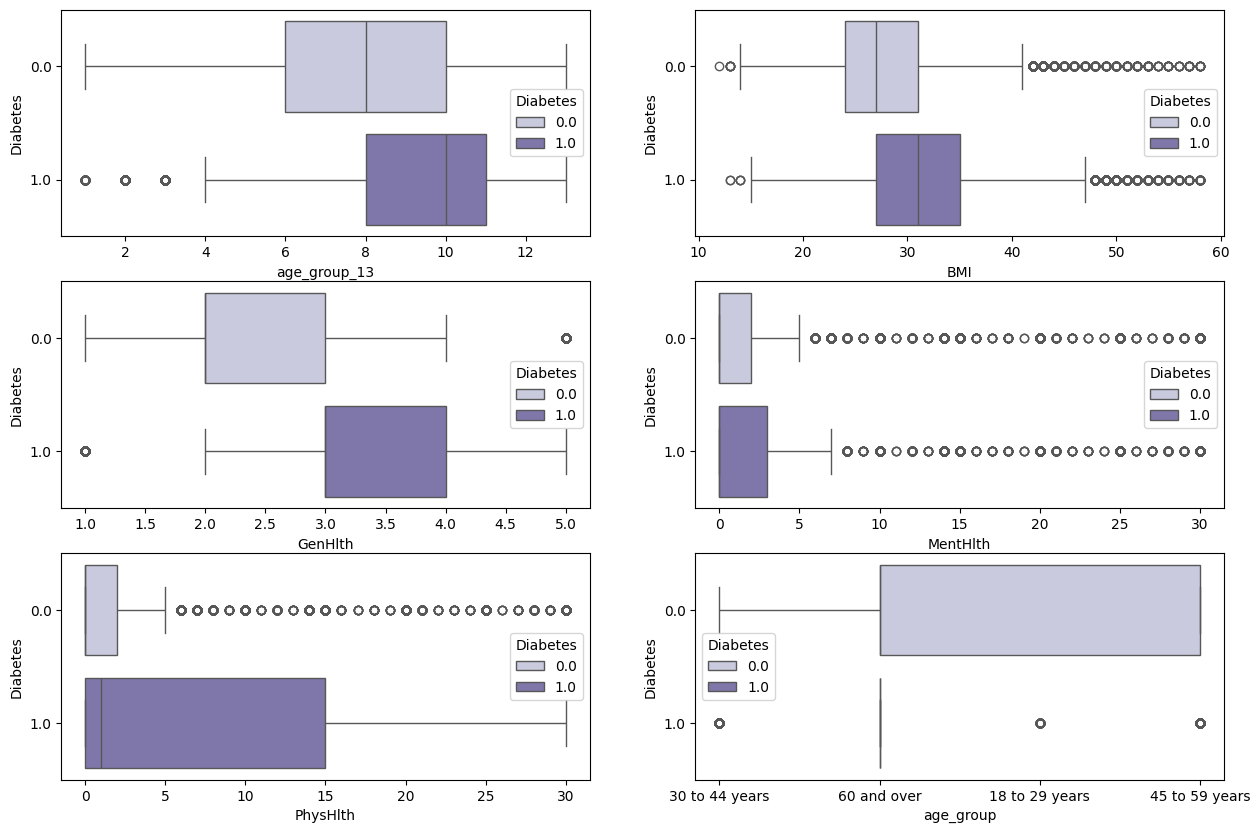
\includegraphics[width=1\linewidth]{raport/graphs/diabetes_boxplots.png}
    \captionsetup{justification=centering}
    \caption{Wykresy pudełkowe zmiennych numerycznych ze zbioru danych dla cukrzycy.}
    \label{fig:enter-label}
\end{figure}

\begin{figure}[H]
    \centering
    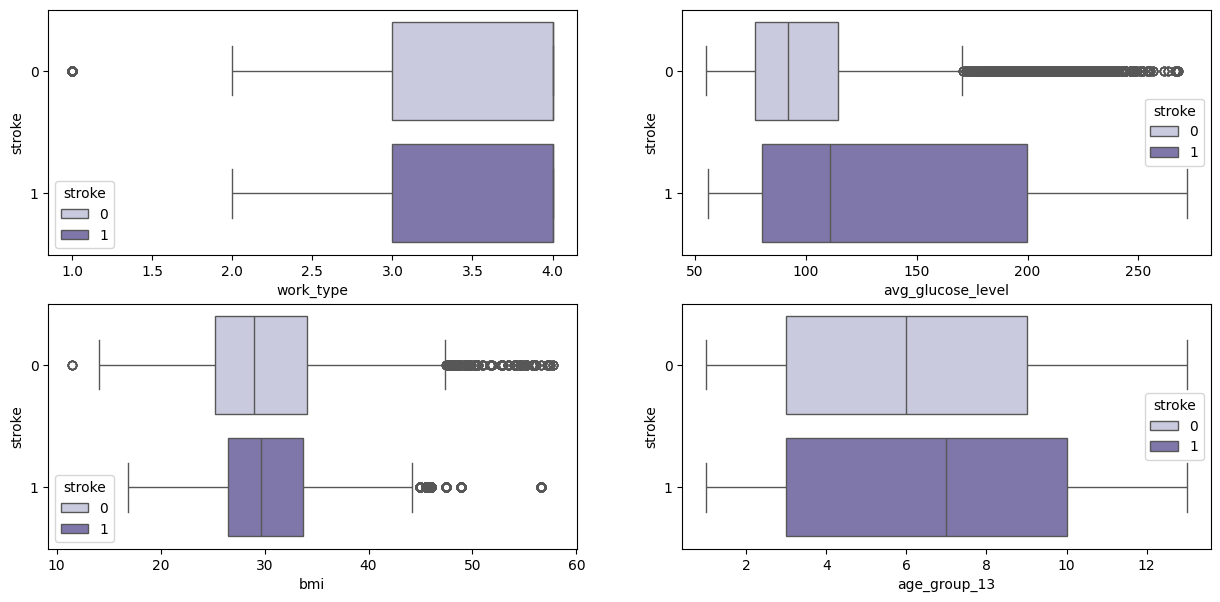
\includegraphics[width=1\linewidth]{raport/graphs/stroke_boxplots.png}
    \captionsetup{justification=centering}
    \caption{Wykresy pudełkowe zmiennych numerycznych ze zbioru danych dla udaru.}
    \label{fig:enter-label}
\end{figure}

\begin{figure}[H]
    \centering
    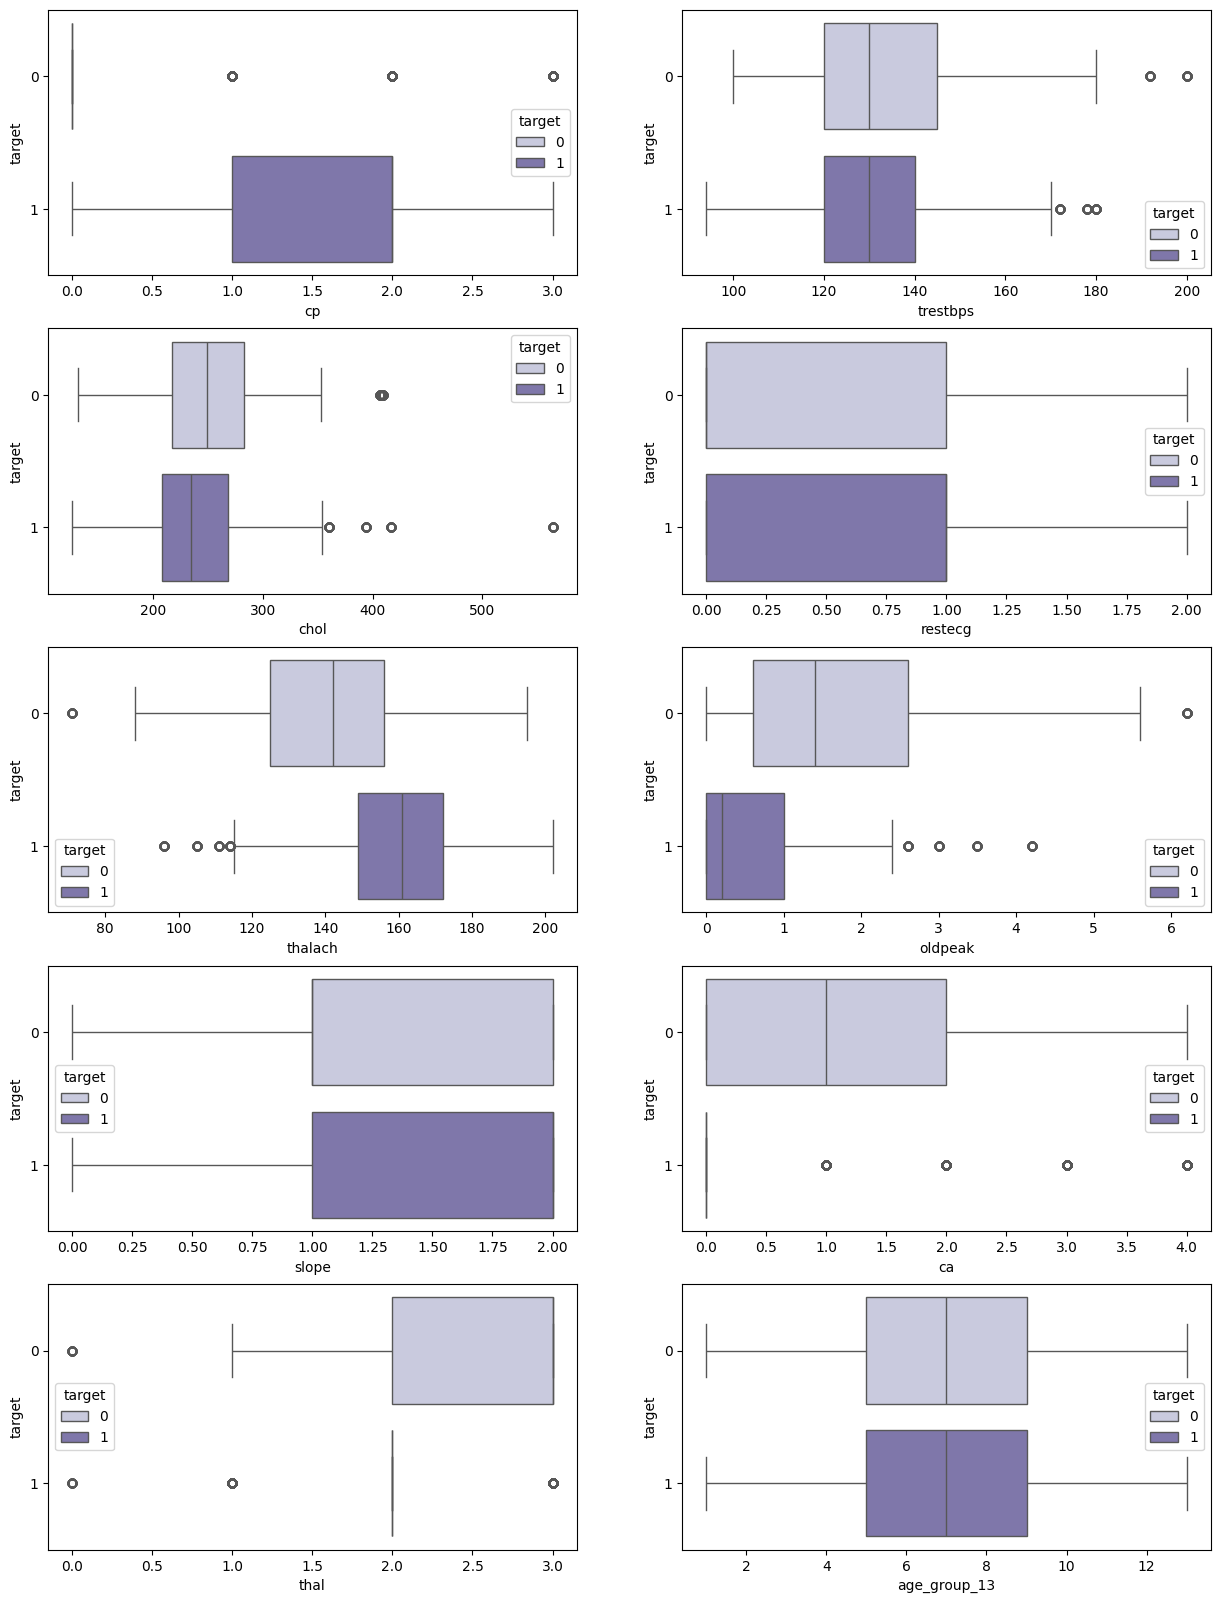
\includegraphics[width=1\linewidth]{raport/graphs/hypertension_boxplot.png}
    \captionsetup{justification=centering}
    \caption{Wykresy pudełkowe zmiennych numerycznych ze zbioru danych dla nadciśnienia.}
    \label{fig:enter-label}
\end{figure}

\newpage
\noindent
Rozkład BMI dla osób z cukrzycą wskazuje na wyższe wartości w porównaniu do osób bez cukrzycy, co sugeruje związek między wyższym BMI a zwiększonym ryzykiem cukrzycy. Ponadto osoby z cukrzycą częściej oceniają swój ogólny stan zdrowia (GenHlth), jak i zdrowie psychiczne (MentHlth) i fizyczne (PhysHlth) na gorszy.

\vspace{8pt}
\noindent
Natomiast osoby z nadciśnieniem mają niższe maksymalne tętno (thalach) w porównaniu z osobami bez nadciśnienia, co może odzwierciedlać wpływ choroby na kondycję serca. Zauważalne są wyższe wartości depresji ST (oldpeak) w EKG u osób z nadciśnieniem, co może wskazywać na związane z nim problemy sercowe.

\vspace{8pt}
\noindent
Istotnie wyższe poziomy glukozy we krwi (avg-glucose-level) są obserwowane u osób, które doświadczyły udaru, co sugeruje silny związek między tymi parametrami. Podobnie, takie osoby częściej znajdują się w kategoriach pracy bardziej stresujących lub mniej aktywnych fizycznie, co może przyczyniać się do zwiększonego ryzyka wystąpienia choroby.

\vspace{8pt}
\noindent
W kolejnym etapie przedstawiono macierze korelacji - narzędzie statystyczne używane do ilościowego określenia i wizualizacji siły i kierunku związku między zmiennymi w zbiorze danych. Każdy element macierzy przedstawia współczynnik korelacji między parami zmiennych, gdzie wartości bliskie +1 lub -1 wskazują na silną korelację dodatnią lub ujemną, a wartości bliskie zeru oznaczają brak zauważalnego związku. Na podstawie wykresów przedstawionych na Rys. 4, 5, 6 dokonano analizy korelacji dla trzech omawianych chorób — cukrzycy, nadciśnienia i udaru. 

\begin{figure}[H]
    \centering
    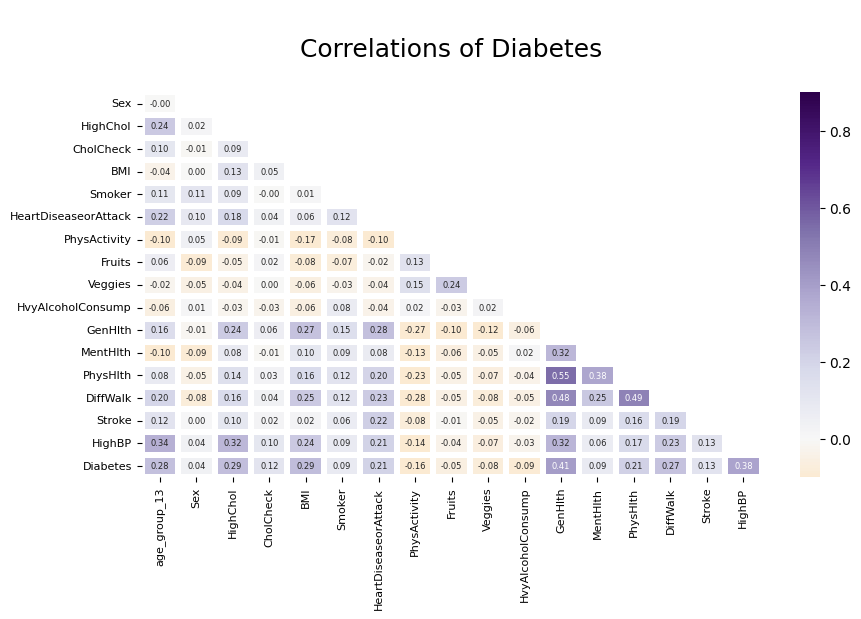
\includegraphics[width=0.85\linewidth]{raport/graphs/diabetes_corr.png}
    \captionsetup{justification=centering}
    \caption{Macierz korelacji dla wszystkich zmiennych ze zbioru danych dla cukrzycy.}
    \label{fig:enter-label}
\end{figure}

\begin{figure}[H]
    \centering
    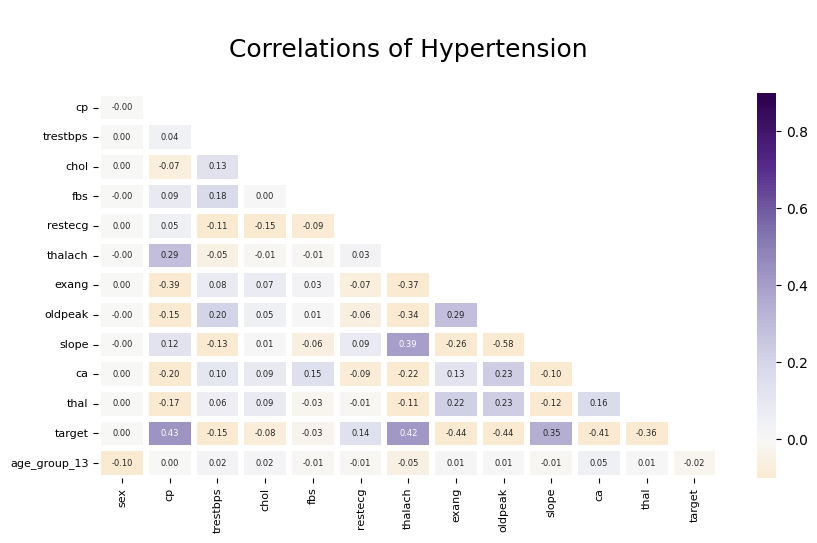
\includegraphics[width=0.85\linewidth]{raport/graphs/hypertension_corr.png}
    \captionsetup{justification=centering}
    \caption{Macierz korelacji dla wszystkich zmiennych ze zbioru danych dla nadciśnienia.}
    \label{fig:enter-label}
\end{figure}

\begin{figure}[H]
    \centering
    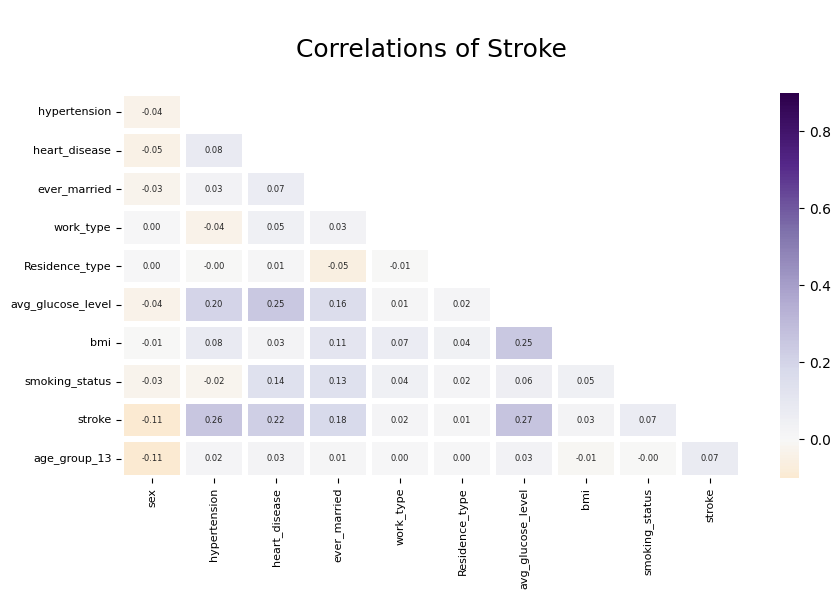
\includegraphics[width=0.85\linewidth]{raport/graphs/stroke_corr.png}
    \captionsetup{justification=centering}
    \caption{Macierz korelacji dla wszystkich zmiennych ze zbioru danych dla udaru.}
    \label{fig:enter-label}
\end{figure}

\newpage
\noindent
W przypadku cukrzycy największą dodatnią korelację wykazują zmienne wskazujące na ogólne samopoczucie pacjenta, takie jak GenHlth z PhysHlth na poziomie 0.55. Podobnym przypadkiem są zmienne PhysHlth i DiffWlk z korelacją 0.49 co odzwierciedla logiczne skojarzenie trudności z chodzeniem przy złym zdrowiu fizycznym. Skupiając się na korelacji zmiennej zależnej (Diabetes) najwyższą wartość wynosi 0.41

\vspace{8pt}
\noindent
Następnie analizująć wykres dla zmiennych związanych z nadciśnieniem najwyższą wartość bezwzględną otrzymano pomiędzy zmiennymi slope, a oldpeak na poziomie -0.58. Jest to spodziewana wartość, ponieważ zmienne te opisują to samo zjawisko, jedynie w różnych punktach na wykresie. Istotniejsze natomiast są korelacje ze zmienna target, opisującą czy u danej osoby stwierdzono nadciśnienie. Na rysunku odznaczają się dwie wartości dla zmiennych: cp - opisuje rodzaj bólu występującego w klatce piersiowej pacjenta oraz thalach - maksymalne zmierzone tętno. 

\vspace{8pt}
\noindent
Na koniec zbadano zbiór opisujący udar. W tym przypadku stwierdzono bardzo mały stopień korelacji między zmiennymi, nie przekraczający bezwzględnie poziomu 0.3. Najwyższą wartość  korelacji 0.25 wykazano między poziomem glukozy we krwi, a ryzykiem udaru, co potwierdza się z analizą wykresów pudełkowych. Ta zależność podkreśla ciekawy związek, który może nie być oczywisty dla przeciętnej osoby. 

\vspace{8pt}
\noindent
Podsumowująć korelacje nie stwierdzono nigdzie silnych powiązań między zmiennymi, które przekroczyły by bewzględną wartość 0.7. Świadczy to o poprawnej strukturze danych, gdzie nie jest konieczne usunięcie danych kolumn.

\vspace{8pt}
\noindent
Ostatnim etapem analizy wykresowej było przedstawienie histogramów częstościowych (ang. countplot) dla cech binarnych z wyodrębnieniem istnienia danej choroby, co pozwala na głębsze zrozumienie, jak poszczególne zmienne mogą wpływać na ryzyko choroby. Histogramy te konkretnie wskazują, czy dana cecha może mieć wpływ na występowanie choroby. Otrzymane wykresy zamieszczono na Rys. 7, 8, 9.


\begin{figure}[H]
    \centering
    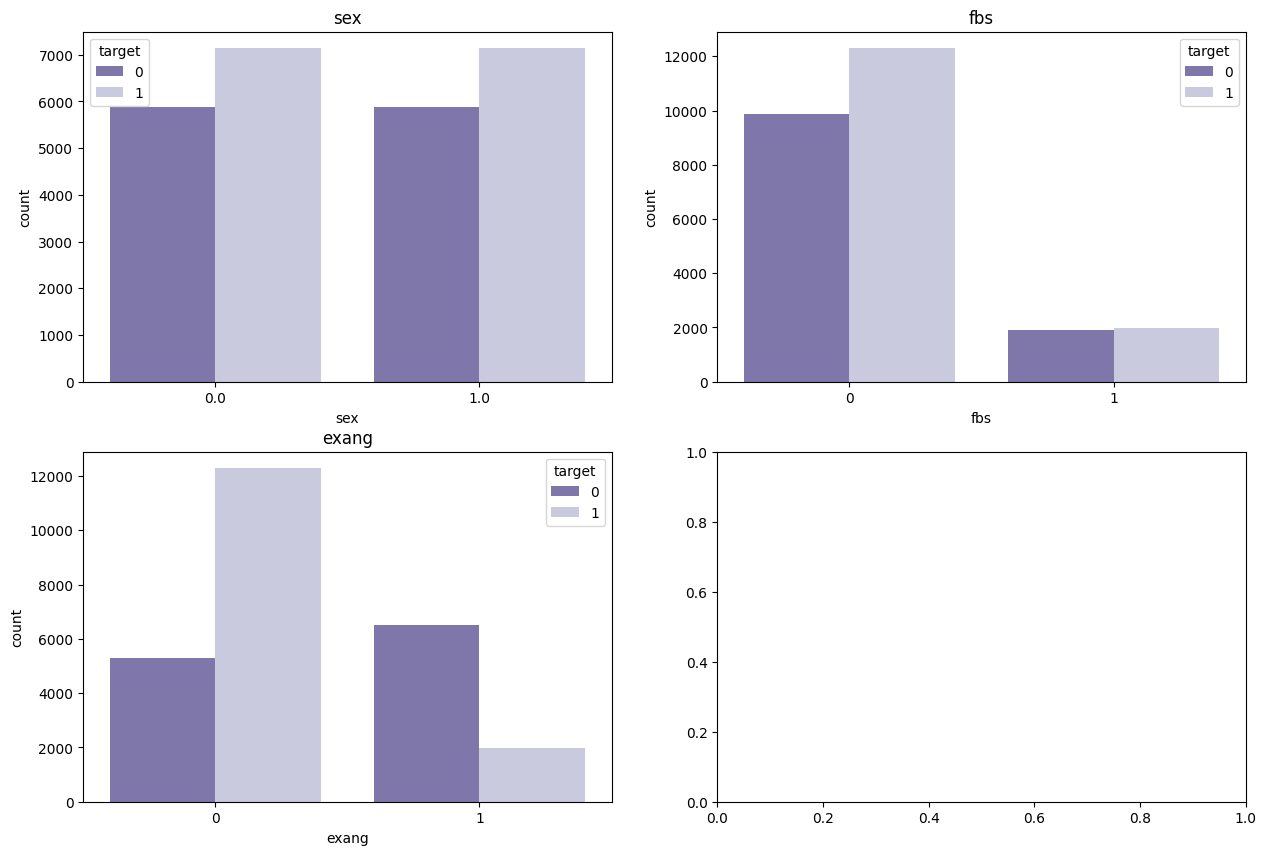
\includegraphics[width=0.85\linewidth]{raport/graphs/hypertension_binary.png}
    \captionsetup{justification=centering}
    \caption{Histogramy częstościowe zmiennych dwuwartościowych ze zbioru danych dla nadciśnienia.}
    \label{fig:enter-label}
\end{figure}

\begin{figure}[H]
    \centering
    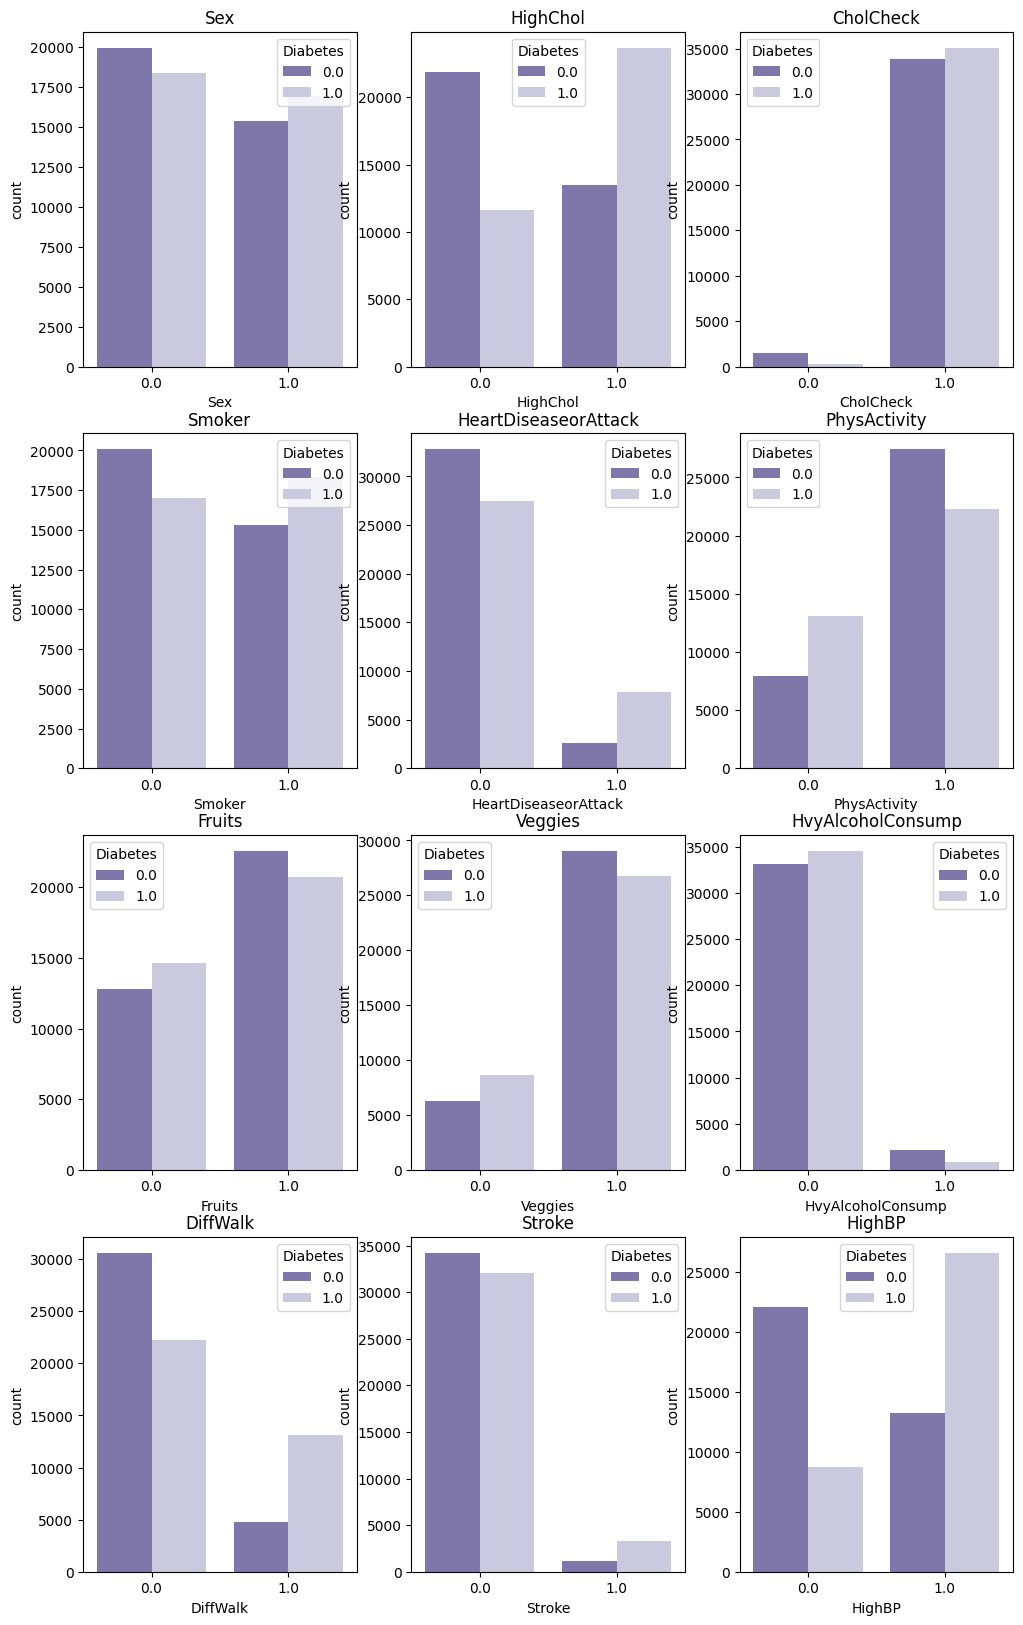
\includegraphics[width=0.8\linewidth]{raport/graphs/diabetes_binary.png}
    \captionsetup{justification=centering}
    \caption{Histogramy częstościowe zmiennych dwuwartościowych ze zbioru danych dla cukrzycy.}
    \label{fig:enter-label}
\end{figure}

\begin{figure}[H]
    \centering
    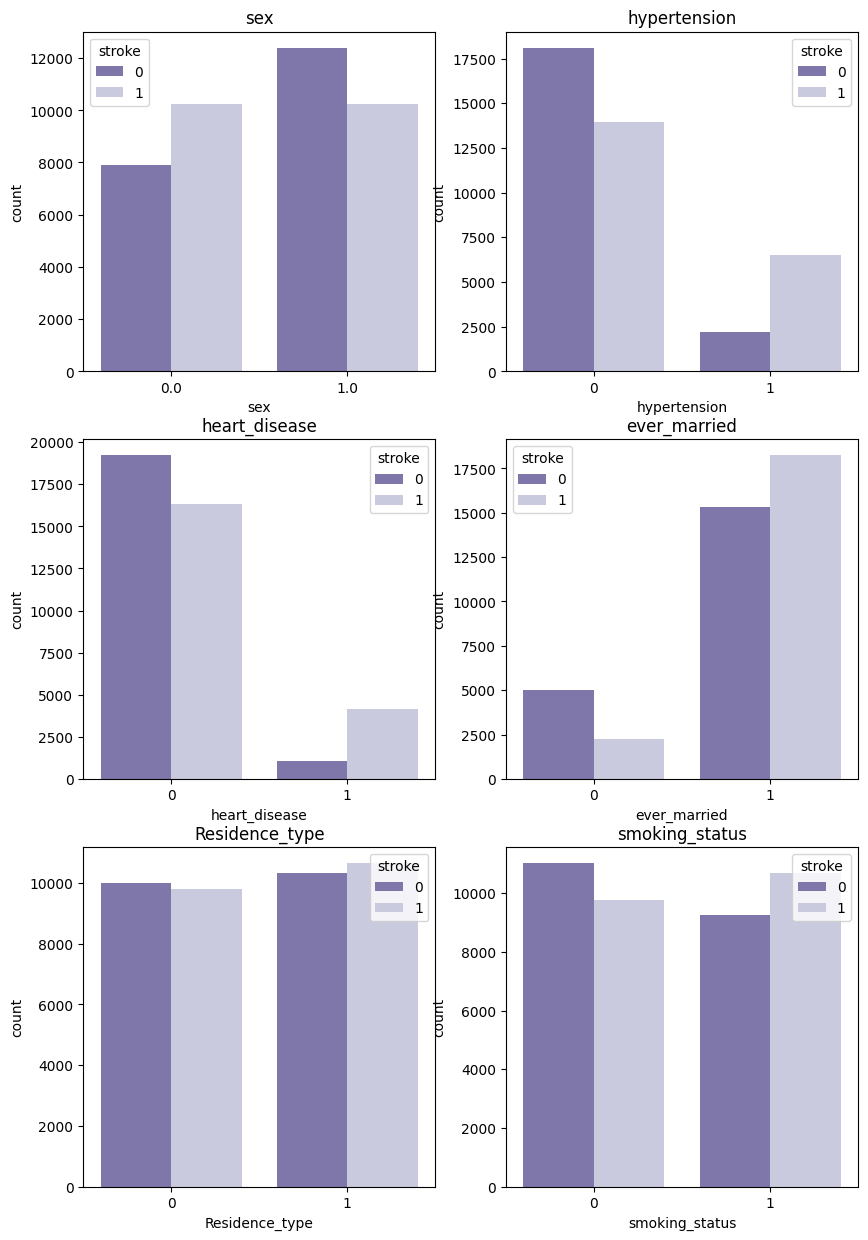
\includegraphics[width=0.8\linewidth]{raport/graphs/stroke_binary.png}
    \captionsetup{justification=centering}
    \caption{Histogramy częstościowe zmiennych dwuwartościowych ze zbioru danych dla udaru.}
    \label{fig:enter-label}
\end{figure}

\newpage
\noindent
Na podstawie wszystkich uzyskanych informacji z analizy wykresów stworzono profile pacjentów którzy znajdują się w grupie ryzyka wystąpienia omawianych chorób.

\vspace{8pt}
\noindent
\textbf{Profil pacjenta z ryzykiem cukrzycy:}
\begin{itemize}
    \itemsep0em 
    \item Wysoki poziom cholesterolu.
    \item Palenie tytoniu (co najmniej 100 papierosów w życiu, czyli około 5 paczek).
    \item Obecność chorób serca, takich jak choroba wieńcowa (CHD) lub zawał mięśnia sercowego (MI).
    \item Brak aktywności fizycznej w ciągu ostatnich 30 dni.
    \item Dieta uboga w warzywa i owoce.
    \item Trudności w poruszaniu się oraz zwiększone ryzyko udaru.
    \item Znaczący wpływ nadciśnienia.
    \item Gorszy stan zdrowia mentalnego i fizycznego.
    \item Podwyższone BMI.
\end{itemize}

\vspace{8pt}
\noindent
\textbf{Profil pacjenta z ryzykiem udaru:}
\begin{itemize}
    \itemsep0em
    \item Starsze osoby często są bardziej narażone.
    \item Obecność chorób serca.
    \item Wysokie ciśnienie krwi.
    \item Czynniki związane ze stanem cywilnym mogą mieć znaczący wpływ.
    \item Wyższe wartości glukozy.
    \item Wyższe BMI.
    \item Historia palenia tytoniu.
\end{itemize}

\vspace{8pt}
\noindent
\textbf{Profil pacjenta z ryzykiem nadciśnienia:}
\begin{itemize}
    \itemsep0em
    \item Ból w klatce piersiowej.
    \item Wyższe wartości skurczowego ciśnienia krwi.
    \item Anomalie w EKG.
    \item Niższe maksymalne tętno.
    \item Ból w klatce piersiowej podczas wysiłku
    \item Niskie wartości depresji odcinka ST.
    \item Mniejsza liczba widocznych naczyń.
\end{itemize}



\newpage

\section{PCA}
\noindent 
PCA (Principal Component Analysis) służy do przekształcania danych wielowymiarowych w przestrzeń o mniejszej liczbie wymiarów, przy jednoczesnym zachowaniu jak największej ilości informacji zawartej w oryginalnych danych. Dzięki temu można uprościć analizę danych i poprawić wydajność algorytmów uczenia maszynowego.

\vspace{8pt}
\noindent 
W kontekście realizowanego projektu PCA będzie stosowane do wybranych modeli predykcyjnych. Wybór liczby składowych, które należy uwzględnić w dalszej analizie, nie może być przypadkowy. Aby podjąć właściwą decyzję, zostanie wykorzystany wykres skumulowanej wariancji wyjaśnionej przez kolejne główne komponenty. Każdy punkt na wykresie pokazuje, ile łącznie wariancji jest wyjaśnione przez daną liczbę głównych składowych. 

\vspace{8pt}
\noindent
Dla celów tego projektu przyjęto, że wyjaśnienie około 95\% wariancji jest wystarczające. PCA przeprowadzono dla każdego zbioru danych:
\begin{itemize}
\item{Zbiór danych dotyczący występowania cukrzycy}

\begin{figure}[H]
    \centering
    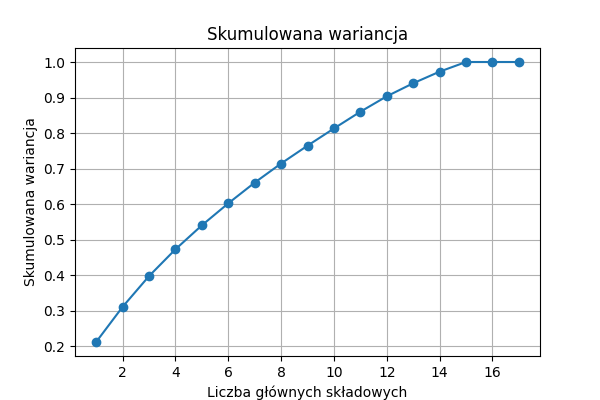
\includegraphics[width=0.8\linewidth]{raport/graphs/skumulowana_wariancja_cukrzyca.png}
    \captionsetup{justification=centering}
    \caption{Wykres skumulowanej wariancji dla cukrzycy.}
\end{figure}

Wykres skumulowanej wariancji dla zbioru o cukrzycy został przedstawiony na Rysunku 10. Widocznych jest 17 głównych składowych. Zdecydowano się na wybór 13 komponentów.

\newpage

\item{Zbiór danych dotyczący występowania nadciśnienia}
\begin{figure}[H]
    \centering
    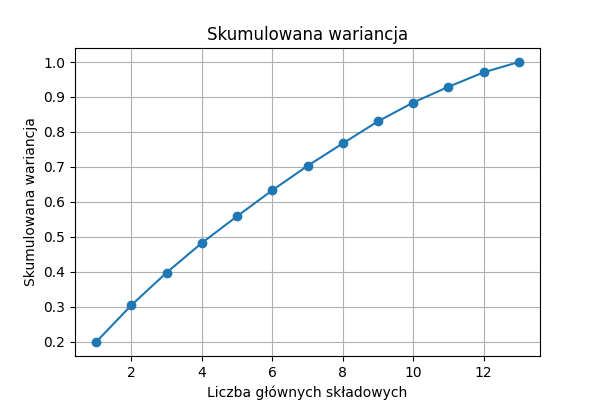
\includegraphics[width=0.80\linewidth]{raport/graphs/skumulowana_wariancja_nadcisnienie.png}
    \captionsetup{justification=centering}
    \caption{Wykres skumulowanej wariancji dla nadciśnienia.}
\end{figure}

Na podstawie Rysunku 11 można zaobserwować 13 głównych składowych dla zbioru danych o nadciśnieniu. Uwzględniając, że wyjaśnienie około 95\% wariancji jest wystarczające, zdecydowano się na zachowanie 11 komponentów.

\item{Zbiór danych dotyczący występowania udaru mózgu}
\begin{figure}[H]
    \centering
    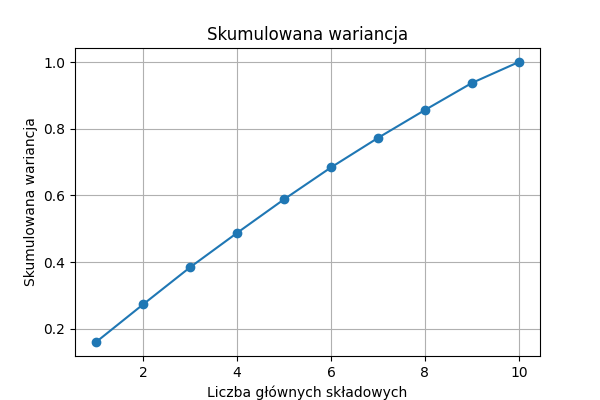
\includegraphics[width=0.80\linewidth]{raport/graphs/skumulowana_wariancja_udar.png}
    \captionsetup{justification=centering}
    \caption{Wykres skumulowanej wariancji dla udaru mózgu.}
\end{figure}
\end{itemize}
Rysunek 12 przedstawia wykres skumulowanej wariancji dla zbioru danych o udarze mózgu. Na jego podstawie można zaobserwować, że 10 głównych składowych wyjaśnia wariancję. W rezultacie zdecydowano się na zachowanie 9 komponentów.

\section{Predykcja wystąpienia choroby}
\subsection{Wybór modeli}
\noindent
W analizie danych medycznych, takich jak zbiory danych dotyczące udarów, nadciśnienia oraz cukrzycy, kluczowym krokiem jest wybór odpowiednich modeli predykcyjnych. Wybrane zostały trzy wybrane modele: regresja logistyczna (Logistic Regression), XGBoost oraz SVM (Support Vector Machine). 

\begin{itemize}
\item{SVM (Support Vector Machine)}

Support Vector Machine (SVM) to model klasyfikacyjny, który szuka hiperplanu maksymalizującego margines między klasami w przestrzeni cech. SVM jest szczególnie skuteczny w przestrzeniach wysokowymiarowych i może używać różnych funkcji jądra (kernel), takich jak liniowa, wielomianowa, RBF (Radial Basis Function), do przekształcania danych.

SVM jest często stosowany w klasyfikacji medycznej, gdy mamy do czynienia z dużą liczbą cech i potencjalnie nieliniowymi granicami decyzyjnymi. Może być używany do przewidywania ryzyka chorób, takich jak udar czy cukrzyca, gdzie granice między zdrowymi a chorymi pacjentami mogą być skomplikowane.

\item{Regresja Logistyczna}

Regresja logistyczna to klasyczny model stosowany do problemów klasyfikacji binarnej. Model ten przewiduje prawdopodobieństwo wystąpienia określonego zdarzenia (np. wystąpienie udaru, nadciśnienia lub cukrzycy) na podstawie zestawu cech (zmiennych niezależnych). Funkcja logistyczna przekształca liniową kombinację zmiennych w przedział [0, 1], co pozwala interpretować wynik jako prawdopodobieństwo.

Regresja logistyczna jest często używana w medycynie ze względu na swoją prostotę i interpretowalność. Jest szczególnie przydatna, gdy istnieje potrzeba zrozumienia wpływu poszczególnych zmiennych na ryzyko wystąpienia choroby. Na przykład, możemy modelować prawdopodobieństwo udaru w zależności od wieku, ciśnienia krwi, poziomu cukru we krwi, itp.

\item{XGBoost}

XGBoost (Extreme Gradient Boosting) to zaawansowany algorytm boostingowy, który tworzy silny model predykcyjny poprzez łączenie wyników słabych uczących (np. drzew decyzyjnych). XGBoost jest znany ze swojej wysokiej wydajności i dokładności.

XGBoost jest często używany do przewidywania wyników w złożonych zbiorach danych medycznych, gdzie relacje między cechami mogą być nieliniowe i skomplikowane. Dzięki swojej zdolności do obsługi brakujących danych i automatycznej optymalizacji hiperparametrów, jest idealnym narzędziem do analizy dużych zbiorów danych, takich jak te dotyczące udarów, nadciśnienia i cukrzycy.
\end{itemize}

\noindent
Wybór odpowiedniego modelu predykcyjnego dla danych medycznych, takich jak te dotyczące udarów, nadciśnienia i cukrzycy, zależy od wielu czynników, w tym interpretowalności, dokładności predykcji oraz złożoności danych. Regresja logistyczna oferuje prostotę i łatwość interpretacji, XGBoost zapewnia wysoką dokładność i zdolność do pracy z dużymi, złożonymi zbiorami danych, a SVM jest skuteczny w analizie danych wysokowymiarowych i nieliniowych. Każdy z tych modeli ma swoje unikalne zalety i ograniczenia, które zostały wzięte pod uwagę przy wyborze najlepszego podejścia do analizy danych medycznych.

\subsection{Ocena modeli}
\noindent
W celu oceny wybranych modeli predykcyjnych posłużono się takimi metrykami jak dokładność, czułość i precyzja.
\subsubsection{Modele podstawowe}
\noindent
W pierwszej kolejności stworzono modele podstawowe dla każdego zbioru danych, które nie uwzględniają strojenia hiperparametrów. 

\begin{figure}[H]
    \centering
    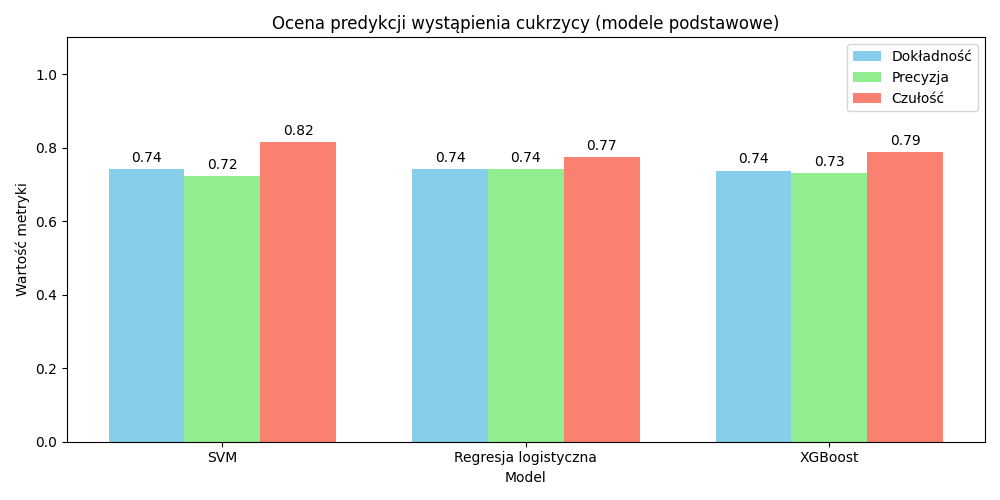
\includegraphics[width=0.90\linewidth]{raport/graphs/cukrzyca_przed.png}
    \captionsetup{justification=centering}
    \caption{Wykres oceny predykcji wystąpienia cukrzycy dla modeli podstawowych.}
\end{figure}

\noindent
Rysunek 13 przedstawia stosowne porównanie modeli przewidujących występowanie cukrzycy. Można zaobserwować, że dokładność kształtuje się na poziomie 74\% dla każdego modelu, precyzja oscyluje w niewielkim zakresie od 72\% do 74\%, zaś czułość prezentuje największe fluktuacje. W kontekście osiągniętej czułości najlepiej poradził sobie model SVM z wynikiem 82\%. 


\begin{figure}[H]
    \centering
    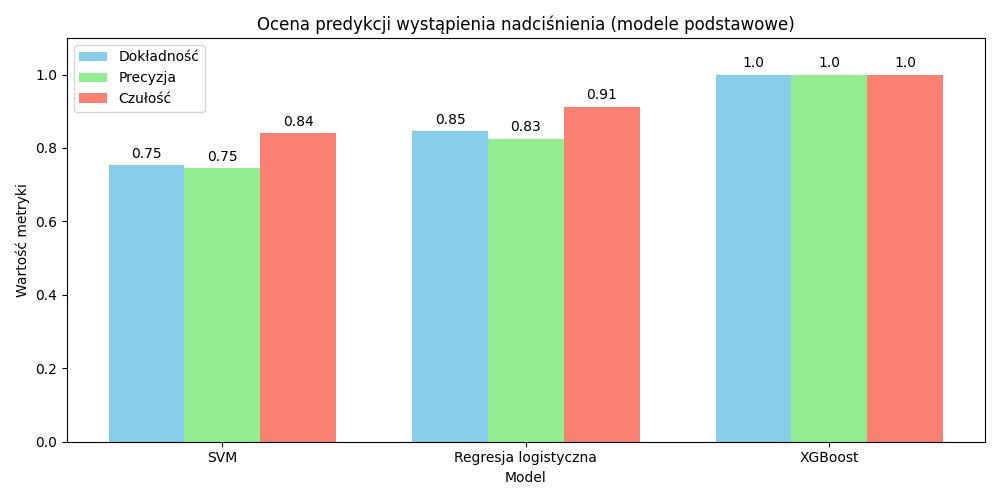
\includegraphics[width=0.90\linewidth]{raport/graphs/nadcisnienie_przed.png}
    \captionsetup{justification=centering}
    \caption{Wykres oceny predykcji wystąpienia nadciśnienia dla modeli podstawowych.}
\end{figure}

\noindent
Na Rysunku 14 można zaobserwować porównanie modeli przewidujących występowanie nadciśnienia. Pierwszą obserwacją jest fakt, że model XGBoost osiągnął wynik 100\% dla każdej z analizowanych metryk. Najsłabiej poradził sobie model SVM, mimo to rezultaty prezentują się lepiej w porównaniu z predykcją występowania cukrzycy.

\begin{figure}[H]
    \centering
    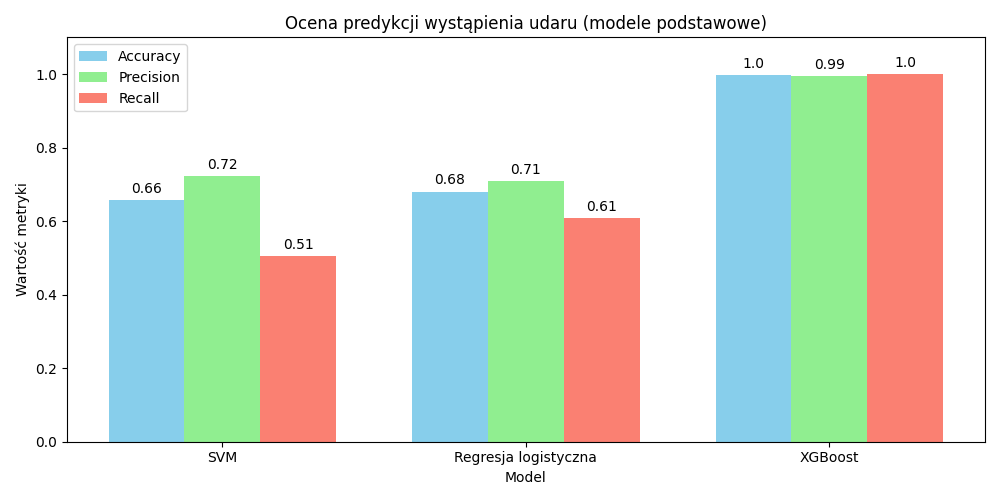
\includegraphics[width=0.90\linewidth]{raport/graphs/udar_przed.png}
    \captionsetup{justification=centering}
    \caption{Wykres oceny predykcji wystąpienia udaru dla modeli podstawowych.}
\end{figure}

\noindent
Ostatnim porównaniem modeli podstawowych jest predykcja występowania udaru mózgu, której wyniki przedstawia Rysunek 15. Po raz kolejny można zaobserwować najlepsze wyniki dla modelu XGBoost. Mimo zbliżonych wartości metryk, to jednak model SVM osiągnął najgorsze wyniki.

\subsubsection{Modele rozszerzone}
\noindent
Następnie modele podstawowe zostały rozszerzone o strojenie hiperparametrów. Proces ten polegał na eksploracji przestrzeni hiperparametrów modelu w celu znalezienia kombinacji, która prowadzi do uzyskania najlepszych rezultatów. W tym celu posłużono się metodą Grid Search (poszukiwanie siatki), która polega na przeszukiwaniu ustalonej siatki możliwych wartości hiperparametrów, aby znaleźć dane kombinacje.

\begin{itemize}
\item{Model przewidujący występowanie cukrzycy}

Dla modelu SVM wykorzystano jądro radialnej funkcji bazowej (RBF) z parametrem regularyzacji C ustawionym na 0.1.

Dla regresji logistycznej zastosowano parametr regularyzacji C równy 0.1, maksymalną liczbę iteracji (max\_iter) ustawioną na 1000 oraz solver 'liblinear'.

Model XGBoost został zbudowany z wykorzystaniem współczynnika uczenia (learning rate) równego 0.01, maksymalną głębokością drzewa (max\_depth) ustawioną na 7, minimalną wagą obserwacji w węźle (min\_child\_weight) ustawioną na 3, oraz parametrem colsample\_bytree na poziomie 0.5, co określa procent kolumn wybieranych losowo podczas budowy każdego drzewa.

\item{Model przewidujący występowanie nadciśnienia}

Dla modelu SVM ponownie wykorzystano jądro radialnej funkcji bazowej (RBF) z parametrem regularyzacji C ustawionym na 0.1.

Dla regresji logistycznej zastosowano parametr regularyzacji C równy 0.1 oraz maksymalną liczbę iteracji (max\_iter) ustawioną na 1000.

Model XGBoost został zbudowany z wykorzystaniem współczynnika uczenia (learning rate) równego 0.01, maksymalną głębokością drzewa (max\_depth) ustawioną na 7, minimalną wagą obserwacji w węźle (min\_child\_weight) ustawioną na 1, oraz parametrem colsample\_bytree na poziomie 0.5.

\item{Model przewidujący występowanie udaru}

Dla modelu SVM wykorzystano jądro radialnej funkcji bazowej (RBF) z parametrem regularyzacji C ustawionym na 10.

Dla regresji logistycznej zastosowano parametr regularyzacji C równy 0.1 oraz maksymalną liczbę iteracji (max\_iter) ustawioną na 1000.

Model XGBoost został zbudowany z wykorzystaniem współczynnika uczenia (learning rate) równego 0.3, maksymalną głębokością drzewa (max\_depth) ustawioną na 5, minimalną wagą obserwacji w węźle (min\_child\_weight) ustawioną na 5, oraz parametrem colsample\_bytree na poziomie 0.5.
\end{itemize}

\noindent
Uzyskane w ten sposób modele rozszerzone po raz kolejny porównano.

\begin{figure}[H]
    \centering
    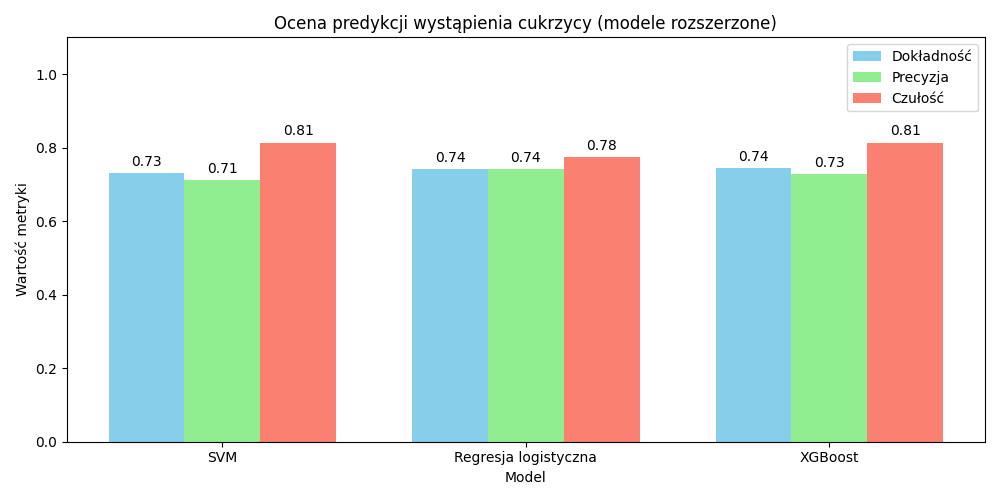
\includegraphics[width=0.90\linewidth]{raport/graphs/cukrzyca_po.png}
    \captionsetup{justification=centering}
    \caption{Wykres oceny predykcji wystąpienia cukrzycy dla modeli rozszerzonych.}
\end{figure}

\noindent
Na podstawie Rysunku 16 można zaobserwować niewielkie zmiany uzyskanych rezultatów dla modeli rozszerzonych w porównaniu z modelami podstawowymi. Wyniki w większości są identyczne, zmiany sięgają maksymalnie rzędu poprawy o dwie jednostki procentowe.

\vspace{8pt}
\noindent
Analizując Rysunek 17, można zauważyć, że wyniki modeli rozszerzonych, przewidujących występowanie nadciśnienia, różnią się od wyników modeli podstawowych. W przypadku modeli regresji logistycznej oraz XGBoost, zmiany w wynikach oscylują na poziomie 1 lub 2 jednostek procentowych. Natomiast dla modelu SVM obserwuje się większe zmiany. Dokładność oraz precyzja modelu SVM poprawiły się o 6 jednostek procentowych, co jest znaczącym wzrostem. Dodatkowo, czułość modelu SVM zwiększyła się o 3 jednostki procentowe. Mimo tych zmian to wciąż model SVM osiąga najgorsze wyniki.

\begin{figure}[H]
    \centering
    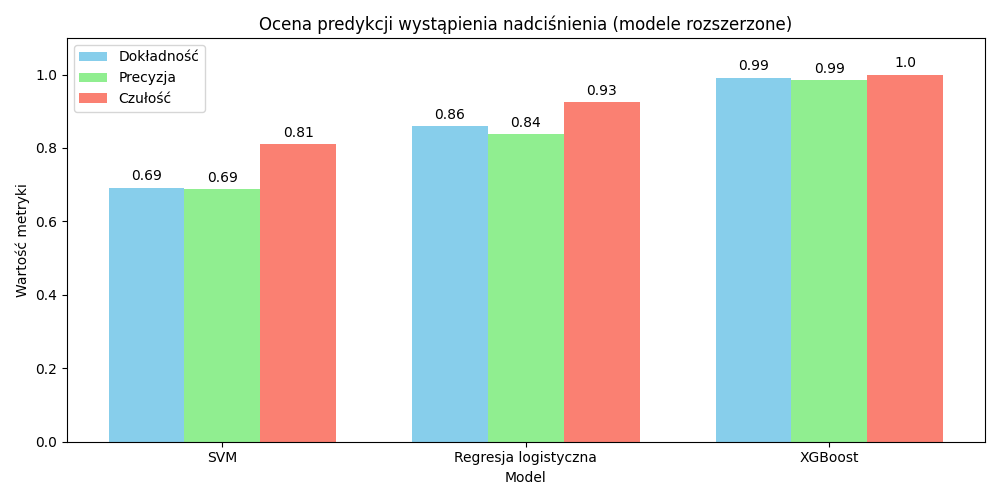
\includegraphics[width=0.90\linewidth]{raport/graphs/nadcisnienie_po.png}
    \captionsetup{justification=centering}
    \caption{Wykres oceny predykcji wystąpienia nadciśnienia dla modeli rozszerzonych.}
\end{figure}


\begin{figure}[H]
    \centering
    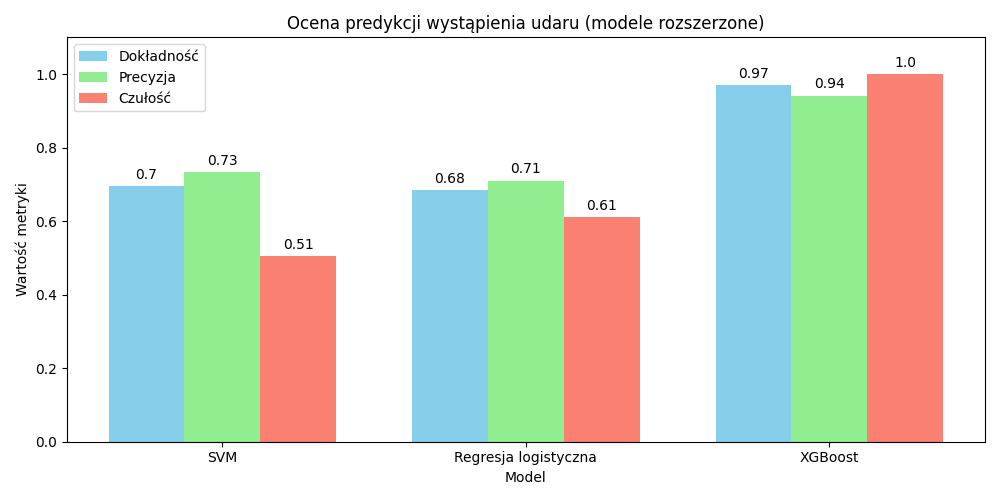
\includegraphics[width=0.90\linewidth]{raport/graphs/udar_po.png}
    \captionsetup{justification=centering}
    \caption{Wykres oceny predykcji wystąpienia udaru dla modeli rozszerzonych.}
\end{figure}

\noindent
Rysunek 18 obrazuje zestawienie modeli rozszerzonych przewidujących występowanie udaru mózgu. Dla modelu XGBoost zaobserwowano pogorszenie wyników w porównaniu z modelem podstawowym. W przypadku regresji logistycznej rezultaty prezentują się na tym samym poziomie. Natomiast dla modelu SVM widoczne jest niewielka poprawa w zakresie dokładności i precyzji. 

\subsubsection{Modele rozszerzone z uwzględnieniem PCA}
\noindent
W ostatniej fazie oceny modeli, zastosowano PCA z wykorzystaniem rozszerzonych modeli. W rozdziale 4 omówiono wybór liczby wykorzystanych komponentów PCA dla każdego zbioru danych. W celach analizy wpływu redukcji wymiarów na wydajność modeli predykcyjnych posłużą wykresy porównawcze.

\begin{figure}[H]
    \centering
    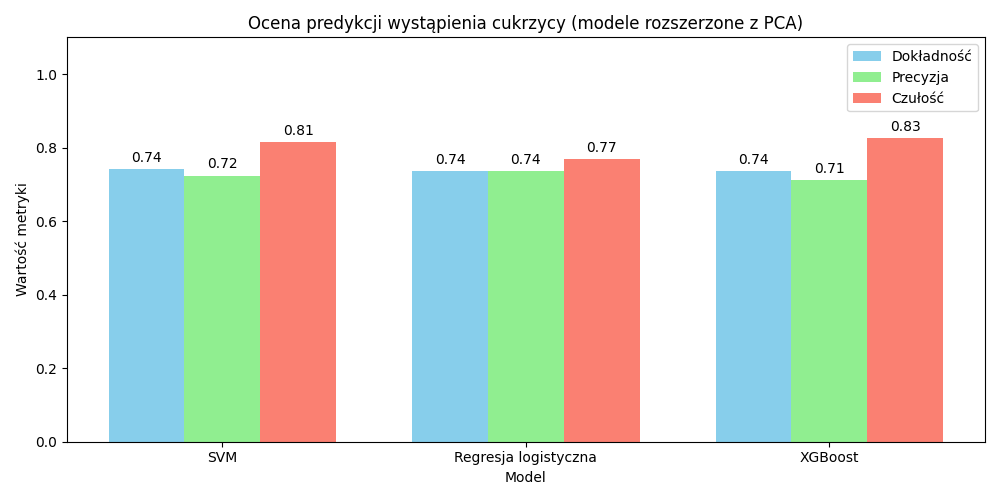
\includegraphics[width=0.86\linewidth]{raport/graphs/cukrzyca_pca.png}
    \captionsetup{justification=centering}
    \caption{Wykres oceny predykcji wystąpienia cukrzycy dla modeli rozszerzonych z PCA.}
\end{figure}

\noindent
Na podstawie Rysunku 19 można zaobserwować niewielkie zróżnicowanie w wynikach osiągniętych przez poszczególne modele. Ponadto, w porównaniu z modelami podstawowymi i rozszerzonymi, zmiany sięgają maksymalnie rzędu 1 do 2 jednostek procentowych. 

\begin{figure}[H]
    \centering
    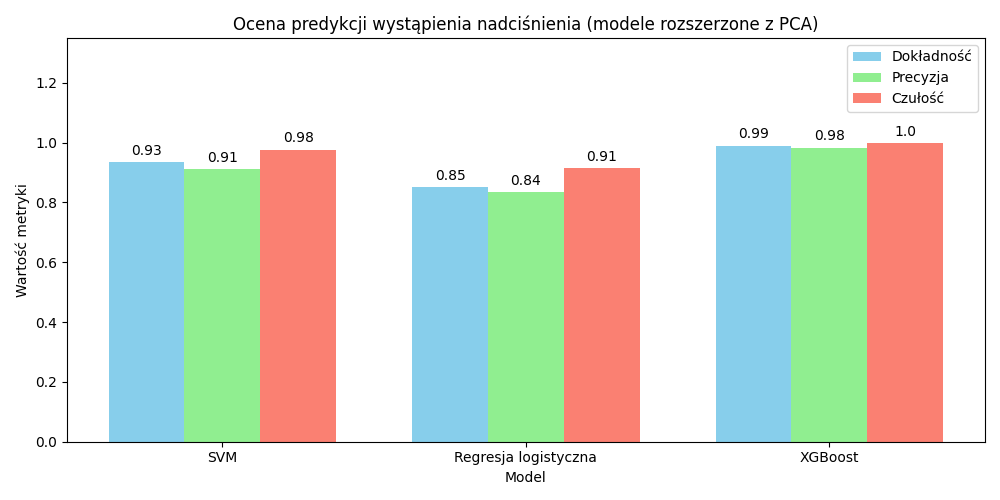
\includegraphics[width=0.86\linewidth]{raport/graphs/nadcisnienie_pca.png}
    \captionsetup{justification=centering}
    \caption{Wykres oceny predykcji wystąpienia nadciśnienia dla modeli rozszerzonych z PCA.}
\end{figure}

\noindent
Analiza Rysunku 20 w zestawieniu z poprzednimi modelami ujawnia znaczącą poprawę wydajności modelu SVM. Zaboserwowano, że dokładność i czułość wzrosły o ponad 20 jednostek procentowych, zaś precyzja zanotowała wzrost o ponad 10 jednostek procentowych. Natomiast zmiany w wydajności pozostałych modeli nie są tak znaczące, oscylując w zakresie od 1 do 2 jednostek procentowych. 

\begin{figure}[H]
    \centering
    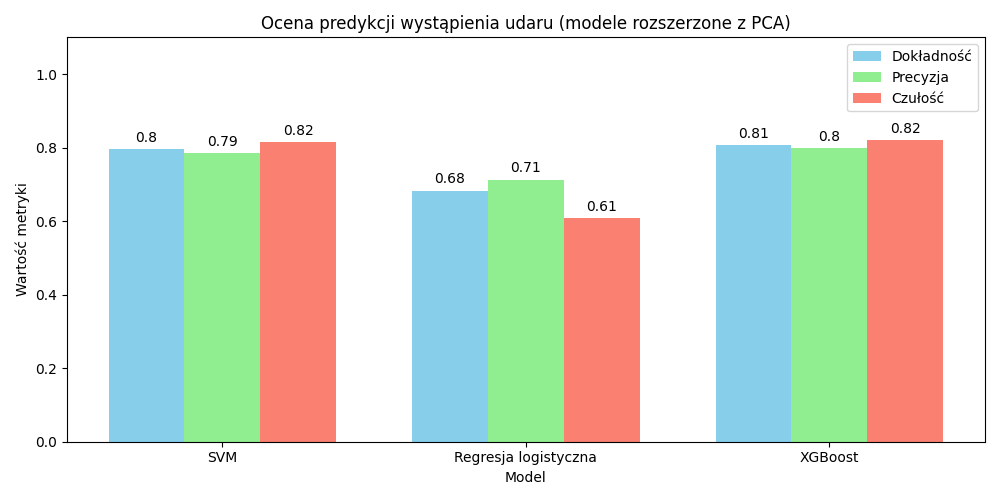
\includegraphics[width=0.90\linewidth]{raport/graphs/udar_pca.png}
    \captionsetup{justification=centering}
    \caption{Wykres oceny predykcji wystąpienia udaru dla modeli rozszerzonych z PCA.}
\end{figure}

\noindent
W przypadku predykcji wystąpienia udaru mózgu dla modeli rozszerzonych z zastosowaniem PCA, której porównanie widoczne jest na Rysunku 21, zaobserwowano zróżnicowane zmiany w wynikach. Model SVM ponownie wykazał znaczącą poprawę. Czułość wzrosła o 30 jednostek procentowych, a pozostałe metryki, takie jak dokładność i precyzja, poprawiły się o około 10 jednostek procentowych. Dla modelu regresji logistycznej nie zauważono żadnych zmian w wynikach. Natomiast model XGBoost wykazał negatywne zmiany w wynikach. Odnotowano spadek o blisko 20 jednostek procentowych dla każdej metryki, co sugeruje, że zastosowanie PCA wpłynęło negatywnie na wydajność modelu.

\section{Analiza czynników ryzyka}
\noindent
Podczas oceny modeli predykcyjnych warto zwrócić uwagę na zidentyfikowanie cech, które mają największy wpływ na przewidywanie danej choroby. Każdy model używa innej metody do określenia znaczenia cech, co pozwala uzyskać szersze spektrum najważniejszych cech. Dzięki temu możliwe jest lepsze zrozumienie, które aspekty są istotne dla prognozowania stanu zdrowia.

\vspace{8pt}
\noindent
Dla każdego z rozszerzonych modeli obliczono znaczenie cech i zwizualizowano je na stosownych wykresach. W pierwszej kolejności dokonano tego dla modeli przewidujących występowanie cukrzycy, co zostało przedstawione na Rysunkach 22, 23, 24.

\vspace{8pt}
\noindent
Dla modelu SVM najważniejszymi cechami okazały się: ogólny stan zdrowia, wyrażony w skali od 1 do 5 (GenHlth), obecność wysokiego ciśnienia (HighBP) oraz obecność wysokiego cholesterolu (HighChol). Dla modelu regresji logistycznej największe znaczenie miały cechy takie jak: kontrola cholesterolu (1-5) (CholCheck), obecność wysokiego ciśnienia (HighBP), obecność wysokiego cholesterolu (HighChol) oraz ogólny stan zdrowia (GenHlth). Natomiast dla modelu XGBoost najważniejszymi czynnikami były wartość BMI, stan zdrowia fizycznego w ciągu ostatnich 30 dni (PhysHlth) oraz wiek zakodowany w 13 kategoriach wiekowych (Age).

\begin{figure}[H]
    \centering
    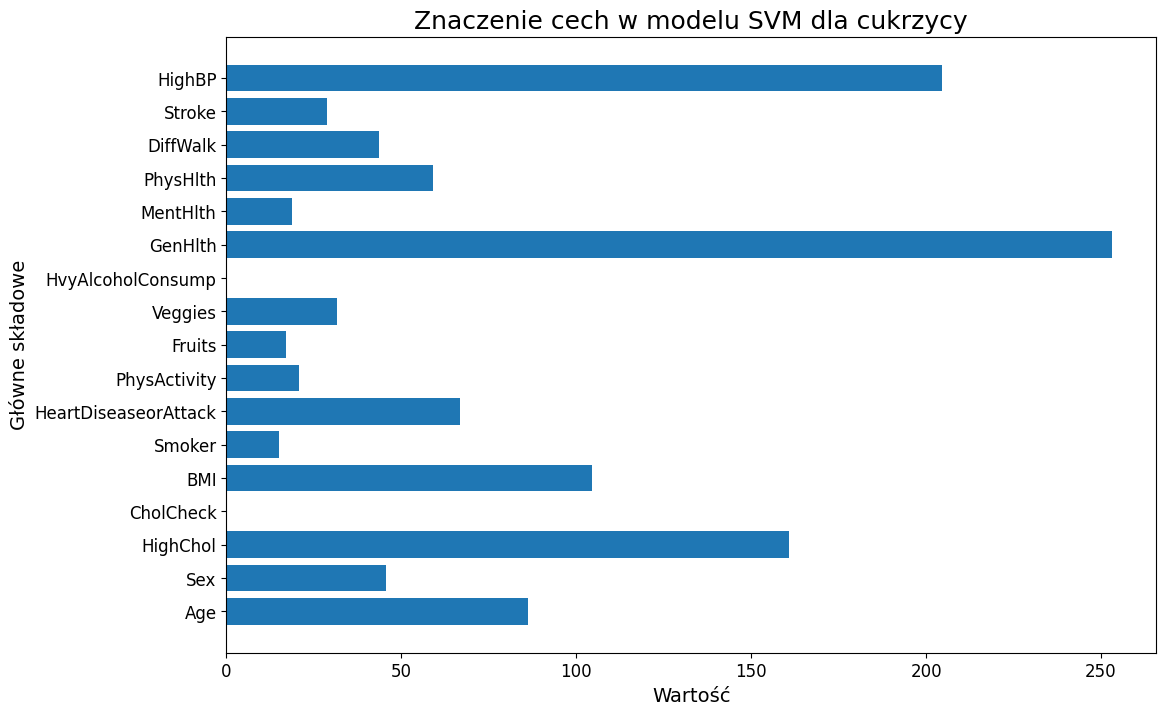
\includegraphics[width=0.90\linewidth]{raport/graphs/cukrzyca_svm.png}
    \captionsetup{justification=centering}
    \caption{Wykres znaczenia cech w modelu SVM dla cukrzycy.}
\end{figure}

\begin{figure}[H]
    \centering
    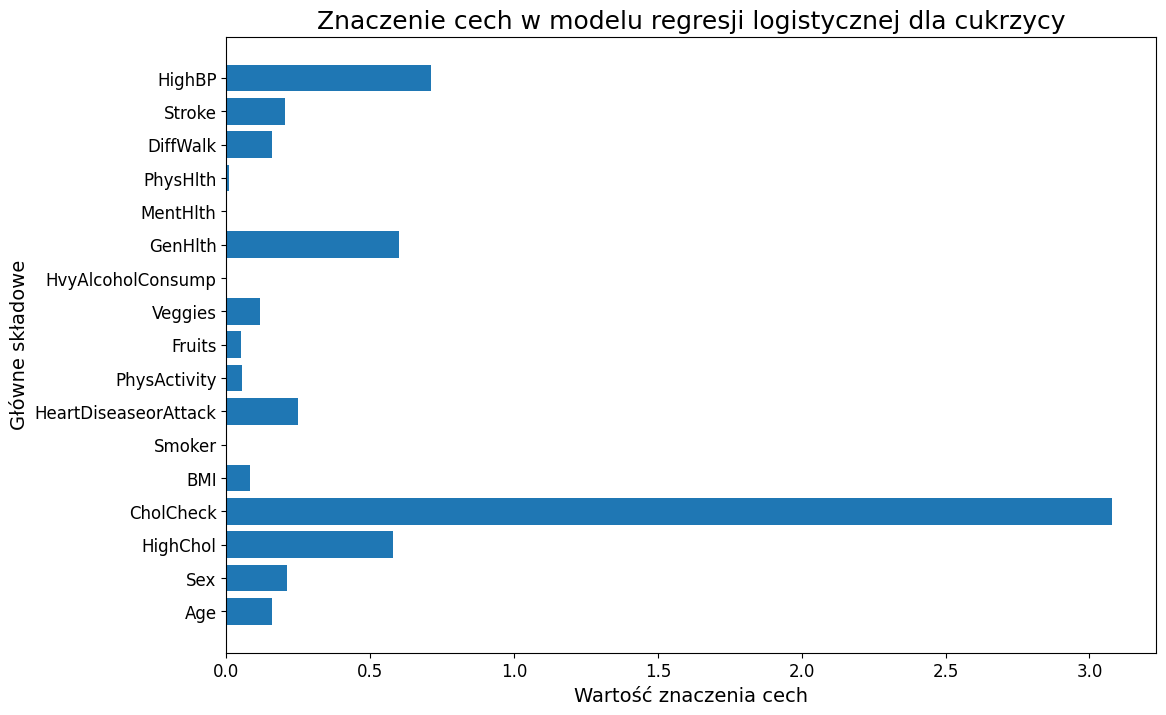
\includegraphics[width=0.90\linewidth]{raport/graphs/cukrzyca_regresja.png}
    \captionsetup{justification=centering}
    \caption{Wykres znaczenia cech w modelu regresji logistycznej dla cukrzycy.}
\end{figure}

\begin{figure}[H]
    \centering
    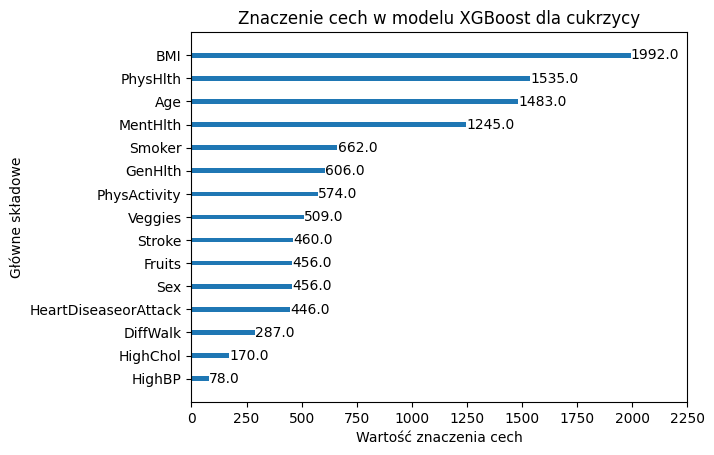
\includegraphics[width=0.90\linewidth]{raport/graphs/cukrzyca_xgb.png}
    \captionsetup{justification=centering}
    \caption{Wykres znaczenia cech w modelu XGBoost dla cukrzycy.}
\end{figure}


\noindent
Tego samego procesu dokonano dla modeli przewidujących występowanie nadciśnienia, co obrazują Rysunki 25, 26, 27.

\begin{figure}[H]
    \centering
    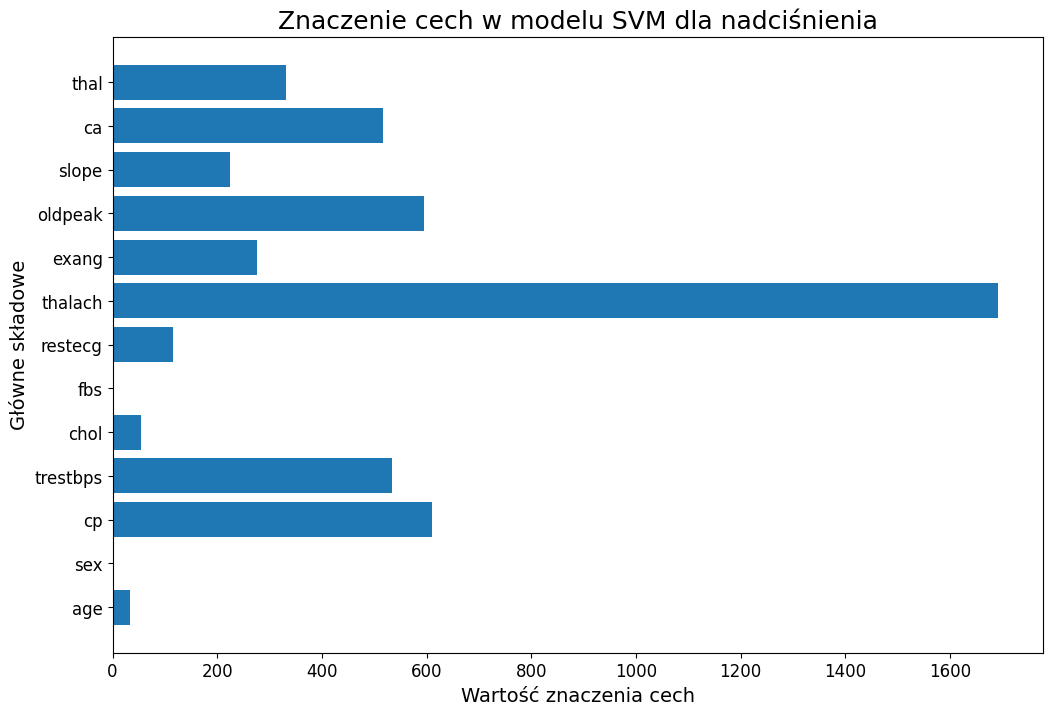
\includegraphics[width=0.90\linewidth]{raport/graphs/nadcisnienie_svm.png}
    \captionsetup{justification=centering}
    \caption{Wykres znaczenia cech w modelu SVM dla nadciśnienia.}
\end{figure}

\begin{figure}[H]
    \centering
    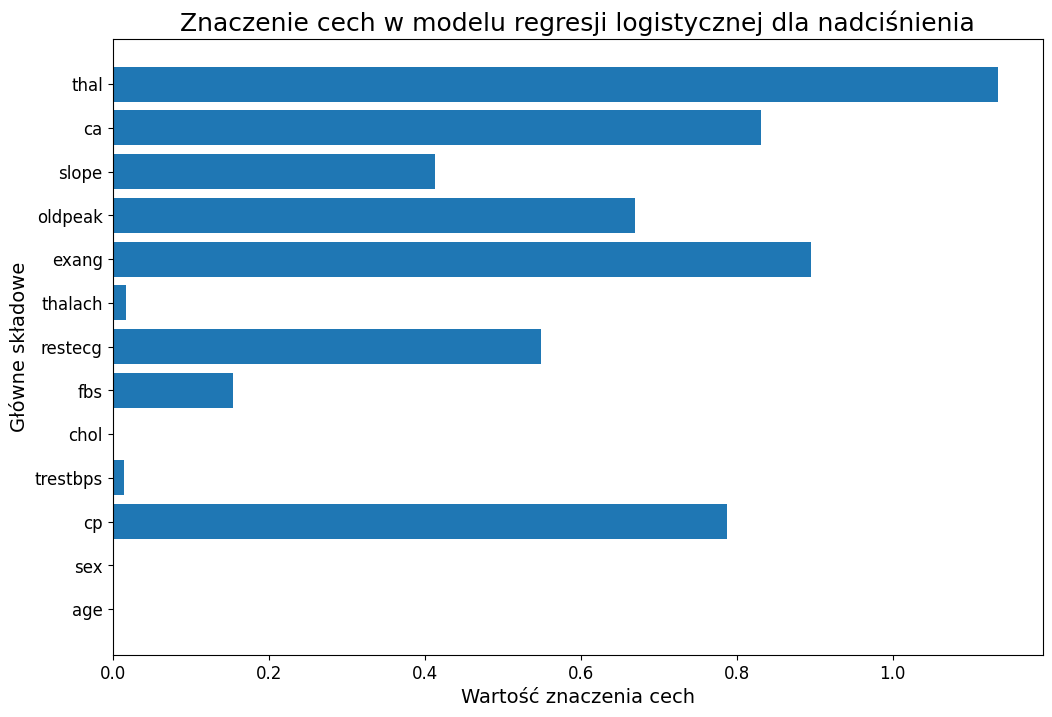
\includegraphics[width=0.90\linewidth]{raport/graphs/nadcisnienie_regresja.png}
    \captionsetup{justification=centering}
    \caption{Wykres znaczenia cech w modelu regresji logistycznej dla nadciśnienia.}
\end{figure}

\begin{figure}[H]
    \centering
    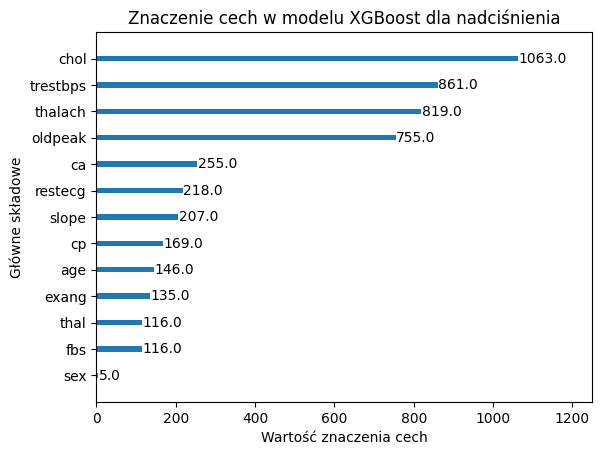
\includegraphics[width=0.90\linewidth]{raport/graphs/nadcisnienie_xgb.png}
    \captionsetup{justification=centering}
    \caption{Wykres znaczenia cech w modelu XGBoost dla nadciśnienia.}
\end{figure}

\newpage
\noindent
W modelu SVM najważniejszymi cechami okazały się: maksymalne tętno (thalach), rodzaj bólu w klatce piersiowej (cp) oraz parametr oldpeak, stosowany przy EKG. Dla regresji logistycznej istotne były zaś: rodzaj defektu w testach thallium (thal), obecność dławicy wysiłkowej (exang) oraz liczba widocznych naczyń na wynikach obrazowania (ca). W modelu XGBoost głównymi cechami okazały się wynik cholesterolu (chol), ciśnienia krwi (trestbps) oraz maksymalne tętno (thalach).

\vspace{8pt}
\noindent
Proces powtórzono dla modeli przewidujących udaru, co obrazują Rysunki 28, 29, 30.

\begin{figure}[H]
    \centering
    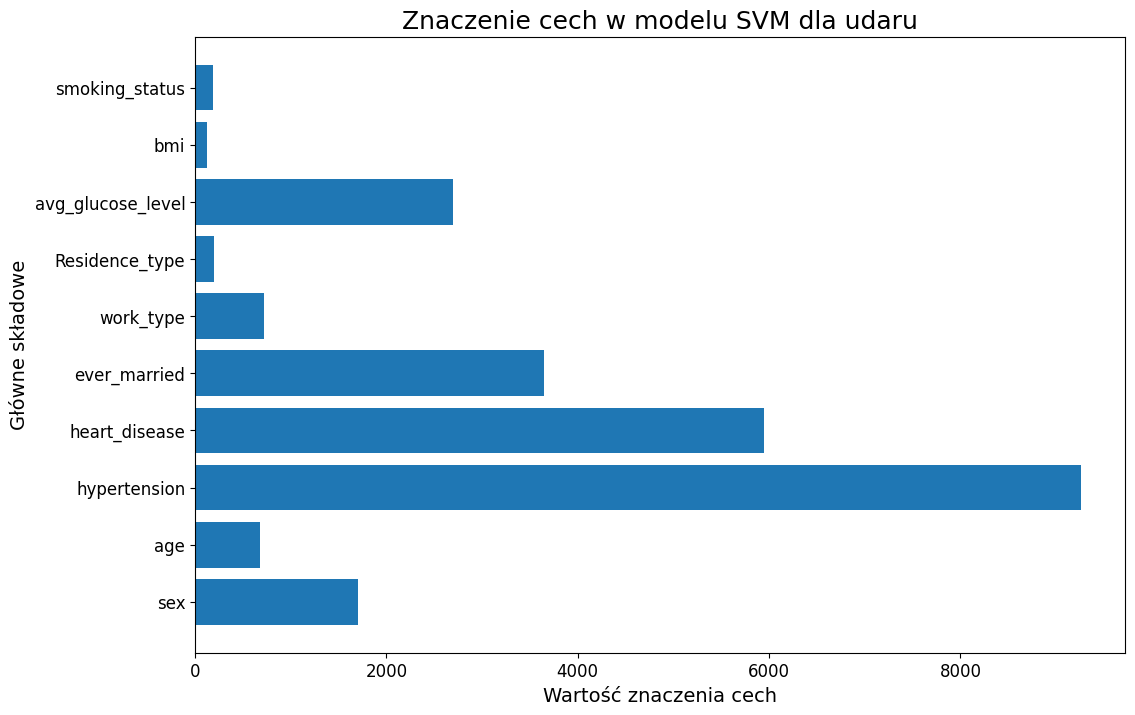
\includegraphics[width=0.90\linewidth]{raport/graphs/udar_svm.png}
    \captionsetup{justification=centering}
    \caption{Wykres znaczenia cech w modelu SVM dla udaru.}
\end{figure}

\begin{figure}[H]
    \centering
    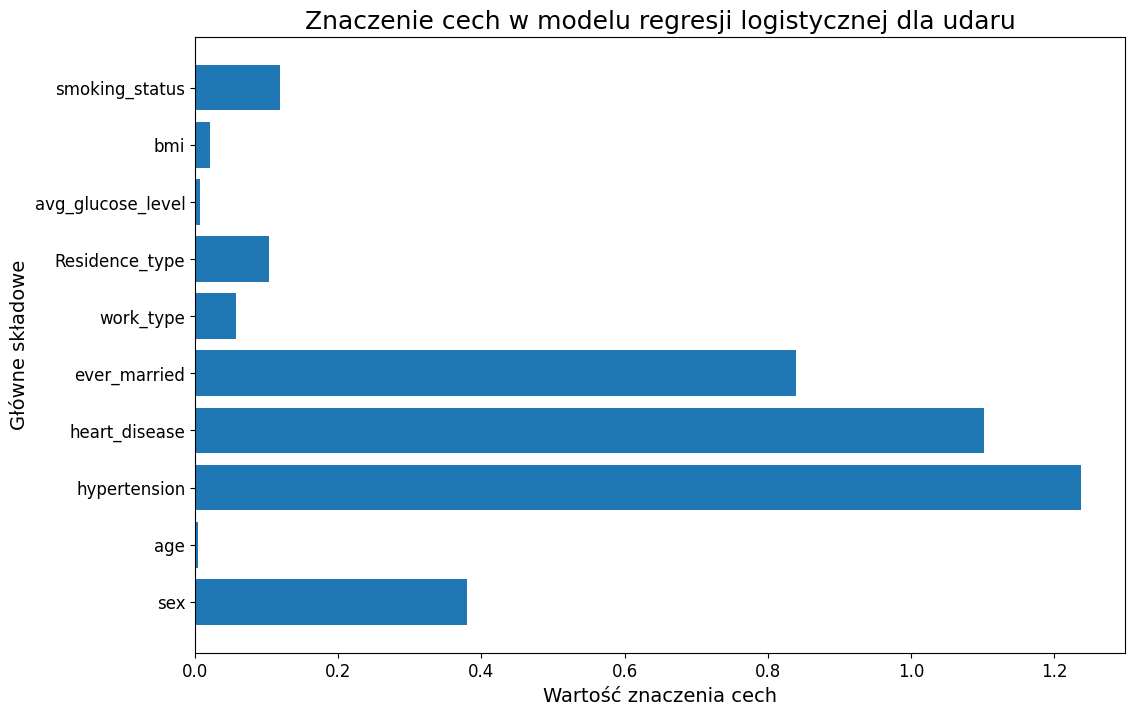
\includegraphics[width=0.90\linewidth]{raport/graphs/udar_regresja.png}
    \captionsetup{justification=centering}
    \caption{Wykres znaczenia cech w modelu regresji logistycznej dla udaru.}
\end{figure}

\begin{figure}[H]
    \centering
    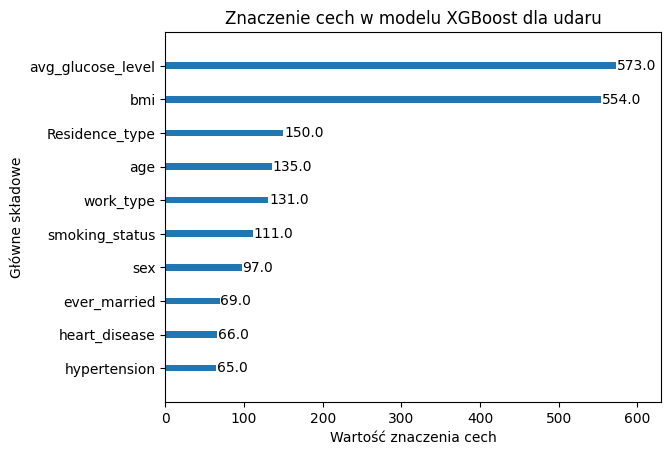
\includegraphics[width=0.90\linewidth]{raport/graphs/udar_xgb.png}
    \captionsetup{justification=centering}
    \caption{Wykres znaczenia cech w modelu XGBoost dla udaru.}
\end{figure}

\noindent
Dla modelu SVM oraz regresji logistycznej kluczowe cechy obejmują występowanie nadciśnienia (hypertension), obecność chorób serca (heart\_disease) oraz informację o stanie cywilnym (ever\_married). Natomiast w przypadku modelu XGBoost wyróżniają się dwie cechy, których wartości znacząco różnią się od pozostałych. Są nimi średni poziom cukru we krwi (avg\_glucose\_level) oraz wskaźnik masy ciała (bmi).

\section{Podsumowanie}
\noindent
Stworzone modele predykcyjne już w wersji podstawowej osiągnęły zadowalające wyniki. Najmniejsze zróżnicowanie w otrzymanych metrykach widoczne jest w przypadku przewidywania cukrzycy. Natomiast dla nadciśnienia i udaru można dostrzec niemal 100\% wydajność modelu XGBoost. Podobna sytuacja występuje w przypadku modeli rozszerzonych, które uwzględniają strojenie hiperparametrów w porównaniu do wersji podstawowych. Osiągnięte wyniki nie różnią się znacząco od tych pierwotnych.

\vspace{8pt}
\noindent
Największe różnice można zauważyć przy zastosowaniu PCA. Mimo że dla cukrzycy nie było znacznych zmian, to dla pozostałych analizowanych chorób zmiany były istotne. Dla nadciśnienia model SVM poprawił się znacznie, nawet o 20 punktów procentowych. Podobnie w przypadku udaru, gdzie ten sam model poprawił się o 30 punktów procentowych pod względem czułości. Pomimo tych pozytywnych zmian, można było zauważyć również negatywny wpływ PCA na model XGBoost, gdzie nastąpił spadek wydajności o blisko 20 punktów procentowych.

\vspace{8pt}
\noindent
Wyjątkowo wysokie metryki modelu XGBoost mogą wynikać z silnej korelacji cech z zmienną zależną, które ten model skutecznie przetwarza. Zaś negatywny wpływ PCA może wynikać z utraty istotnych informacji oraz zmiany struktury i relacji między cechami, które są istotne dla działania XGBoost.

\vspace{8pt}
\noindent
Modele różniły się między sobą uzyskanymi metrykami oraz reakcją na zmiany takie jak PCA, co wynika z ich różnej struktury. Kolejną zauważalną różnicą były czynniki, które każdy z modeli analizował w różnym stopniu. Największe podobieństwa występowały między modelem SVM a regresją logistyczną. W przypadku cukrzycy i udaru najważniejsze cechy były niemal identyczne dla obu modeli. Wyjątkiem było nadciśnienie, gdzie najbardziej istotne cechy różniły się znacząco między tymi dwoma modelami. Natomiast model XGBoost w każdym przypadku skupiał się na zupełnie innych zmiennych, co odzwierciedla jego unikalne podejście do analizy danych.

\begin{thebibliography}{9}
\end{thebibliography}

\end{document}
